% 版式参考公开中文技术报告单栏模板：
% https://www.overleaf.com/latex/templates/zhong-wen-ji-zhu-bao-gao-latexmo-ban-dan-lan-cjc-xelatex/tcnttxfsqykx
% 中文章节、目录和字体由 CTeX 的 ctexrep 文档类提供。
\documentclass[UTF8,oneside,openany,zihao=-4,scheme=chinese,fontset=windows]{ctexrep}
\usepackage[a4paper,top=2.6cm,bottom=2.5cm,left=2.6cm,right=2.4cm]{geometry}
\usepackage{graphicx}
\usepackage{booktabs}
\usepackage{longtable}
\usepackage{tabularx}
\usepackage{array}
\usepackage{makecell}
\usepackage{multirow}
\usepackage{enumitem}
\usepackage{tikz}
\usepackage{caption}
\usepackage{float}
\usepackage{url}
\usepackage{hyperref}
\usepackage[backend=biber,style=gb7714-2015,sorting=none,gbnamefmt=lowercase,maxbibnames=8]{biblatex}

\usetikzlibrary{arrows.meta,positioning,calc,shapes.geometric}
\addbibresource{references.bib}

\hypersetup{
  hidelinks,
  pdfauthor={MediFlow},
  pdftitle={MediFlow 技术报告},
  pdfsubject={基于 MCP 的医疗数据处理与知识分析系统}
}
\urlstyle{same}

\setlength{\parindent}{2em}
\setlength{\parskip}{0pt}
\linespread{1.35}
\setlist[itemize]{leftmargin=2.2em,itemsep=0.18em,topsep=0.35em}
\setlist[enumerate]{leftmargin=2.4em,itemsep=0.18em,topsep=0.35em}
\renewcommand{\arraystretch}{1.22}

\ctexset{
  chapter={
    format=\raggedright\zihao{2}\bfseries,
    beforeskip=12pt,
    afterskip=18pt,
    fixskip=true
  },
  section={
    format=\raggedright\zihao{3}\bfseries,
    beforeskip=1.1\baselineskip,
    afterskip=0.55\baselineskip,
    fixskip=true
  },
  subsection={
    format=\raggedright\zihao{4}\bfseries,
    beforeskip=0.8\baselineskip,
    afterskip=0.35\baselineskip,
    fixskip=true
  }
}

\captionsetup{
  font=small,
  labelfont=bf,
  labelsep=quad,
  skip=6pt
}

\pagestyle{plain}

\newcolumntype{Y}{>{\raggedright\arraybackslash}X}
\newcolumntype{C}[1]{>{\centering\arraybackslash}p{#1}}
\newcolumntype{L}[1]{>{\raggedright\arraybackslash}p{#1}}

\newcommand{\repoPath}[1]{{\small\path{#1}}}

\tikzset{
  reportbox/.style={
    rectangle,
    draw=black,
    fill=white,
    line width=0.65pt,
    rounded corners=1.2pt,
    align=center,
    minimum height=10mm,
    inner sep=4pt,
    font=\small
  },
  reportdata/.style={
    cylinder,
    shape border rotate=90,
    aspect=0.23,
    draw=black,
    fill=white,
    line width=0.65pt,
    align=center,
    minimum height=12mm,
    minimum width=28mm,
    font=\small
  },
  reportarrow/.style={
    -{Latex[length=1.9mm,width=1.2mm]},
    line width=0.65pt,
    draw=black,
    shorten <=2pt,
    shorten >=2pt
  },
  reportline/.style={
    line width=0.65pt,
    draw=black,
    shorten <=2pt,
    shorten >=2pt
  }
}

\AtBeginBibliography{%
  \footnotesize
  \setlength{\bibitemsep}{0.10\baselineskip}
}

\AtEveryBibitem{%
  \ifentrytype{online}{}{\clearfield{url}}%
}


\begin{document}

\begin{titlepage}
  \centering
  \vspace*{3.4cm}

  {\zihao{-0}\bfseries MediFlow\par}
  \vspace{0.9cm}
  {\zihao{2}\bfseries MediFlow：面向医疗数据治理、知识构建与自然语言分析的智能体系统\par}
  \vspace{0.25cm}
  {\zihao{2}\bfseries 基于 Nexent 与 DataMate 的工程实现报告\par}

  \vspace{2.4cm}
  \rule{0.58\textwidth}{0.8pt}\par
  \vspace{0.75cm}
  {\zihao{1}\bfseries 技术报告\par}
  \vspace{0.75cm}
  \rule{0.58\textwidth}{0.8pt}\par

  \vfill
  {\zihao{4}ModelEngine 开源项目贡献赛作品\par}
  \vspace{2.2cm}
\end{titlepage}

\pagenumbering{Roman}
\begingroup
\linespread{1.0}\selectfont
\tableofcontents
\endgroup
\clearpage

\chapter*{\makebox[\textwidth][c]{摘\quad 要}}
\addcontentsline{toc}{chapter}{摘要}

医疗资料同时包含自由文本、表格、JSON 记录和 PDF 文档。赛题要求智能体完成数据处理、知识构建和自然语言分析，并使各阶段产物可查询、可校验。MediFlow 以 Nexent 为对话入口，通过 MCP 将智能体的任务级规划与 DataMate 的数据集、算子和任务执行连接起来。

系统沿“数据处理→知识构建→分析查询”组织三项任务。任务一保留输入数据的字段、键名和记录边界，将文本治理结果登记为交付数据集。任务二将清洗记录转为实体、关系和三元组，经离线优先的级联抽取、否定识别、可靠性分级和来源证据校验后写入图谱。任务三由统一分析服务承接 Nexent 对话和 Web 工作台入口，根据医疗语义和数据表生成查询计划，在只读连接、允许查询对象清单和执行时限约束下形成分析结果。

三个智能体均采用“智能体选择任务级工具、服务确定阶段内执行路径”的分工。工具调用负责表达任务意图，服务和算子负责完成确定性处理，来源、运行状态和分析结果通过统一标识关联。

在固定留出集上，离线实体识别使用 2\,500 条 CMeEE 样本，F1 为 37.70\%；离线关系抽取使用 1\,793 条 CMeIE 样本，F1 为 14.31\%。任务三另以实际分析库构建 133 道 NL2SQL 题，固定测试集的初始配置执行准确率为 61.3\%，优化配置验证结果为 95.7\%。报告同时给出抽取质量、查询准确率、在线响应时间和数据规模，使三项任务的处理效果与服务能力具有统一的量化依据。

\vspace{0.7em}
\noindent\textbf{关键词：}
医疗数据治理；MCP；智能体；知识图谱；自然语言数据分析；DataMate；Nexent

\clearpage


\pagenumbering{arabic}
\chapter{项目背景与系统定位}

\section{赛题要求与业务背景}

ModelEngine 面向数据处理、知识生成和智能体应用提供开源工具链。DataMate 管理数据集、文件和算子任务，Nexent 管理智能体配置、工具绑定和对话执行。作品需要在两套平台之间建立可运行的医疗业务链路，完成数据处理、知识构建与问答、数据分析三个任务，并交付可核验的结果。

医疗资料同时包含自由文本、结构化表格、JSON 嵌套对象和 PDF 文档。实体、关系和来源信息分散在不同记录中，分析结果还需要以文字回答、统计图表和文件形式交付。

MediFlow 围绕三个赛题问题组织工程方案。数据处理阶段由智能体判断探查、处理和状态查询意图，服务根据数据状态选择格式处理链；知识构建阶段将记录转换为带来源的实体关系，经分级和校验后写入图谱；分析阶段把用户问题映射到图谱事实、分析表或只读查询，并生成可追踪的成果记录。

系统当前处理医学知识资料和聚合统计，定位为面向知识资料的工程系统。现有数据没有可用时间维度，分析结果按知识条目和关系事实解释。本文的系统对象包括三部分：MediFlow 提供 MCP 工具和医疗领域处理服务，Nexent 中的三个智能体负责任务级规划，DataMate 负责数据集和算子执行。


\section{MediFlow 系统定位}

MediFlow 是连接 Nexent 与 DataMate 的医疗数据处理与知识分析系统。系统把 DataMate 的数据集、算子和任务接口封装为 MCP 工具，再由领域服务补充格式路由、实体关系校验、图谱写入和只读查询规则。Nexent 中的三个智能体分别面向数据处理、知识图谱和数据分析；它们共享服务入口，并按职责限制可见工具和回复范围。

本文后续统一使用以下称谓：MediFlow 指本项目系统，MediFlow 服务指提供 MCP 接口的服务进程，智能体指 Nexent 中的任务配置，工具指智能体可调用的 MCP 接口，算子指 DataMate 执行的单步数据变换。系统输出中的“处理记录”保存文件状态、阶段统计和质量字段；“来源记录”保存数据集、文件和知识来源；“分析结果记录”保存问题、查询计划、SQL、数据行、图表配置和来源信息。

\section{数据驱动的业务链路}

作品沿“数据处理→知识构建→分析查询”的业务链路组织三个阶段。数据处理阶段接入原始资料，完成文本治理和结构保持后登记交付数据集；知识构建阶段读取交付数据集，抽取实体关系，经分级、校验和去重后写入知识图谱，并刷新分析库；分析查询阶段读取图谱和分析库，生成回答、图表和导出文件。

\chapter{作品整体设计方案}

\section{总体方案与平台边界}

MediFlow 把任务理解、领域编排和平台执行分成三个边界。Nexent 识别用户目标并选择任务级工具；MediFlow 校验参数、读取数据状态并选择处理流程；DataMate 执行数据集任务和单步算子，知识库与分析库负责持久化。当前三个智能体分别配置 5、11 和 8 项工具，去重后形成 17 个工具名称；工具在不同角色之间复用，但每个角色只暴露与其职责相关的入口。

三个阶段通过四类标识衔接：DataMate 数据集标识确定输入和交付数据集；任务一运行标识跟踪后台处理；任务二来源标识和记录标识定位文件与图谱记录；任务三分析标识关联问题、查询结果、图表和导出文件。
用户既可分别使用三个智能体，
也可将任务一产生的数据集直接交给任务二，
再由任务三读取图谱及分析表完成查询。

\section{系统分层与平台边界}

图~\ref{fig:architecture} 给出了作品的五层结构。
交互层包含 Nexent 对话入口和可视化工作台；智能体层按数据处理、知识构建和分析查询划分职责；接口层提供 MCP 工具和工作台业务接口；服务层由 DataMate 平台、医疗知识服务和分析服务组成；数据层保存交付数据集、知识图谱、分析数据库和导出文件。

\begin{figure}[H]
\centering
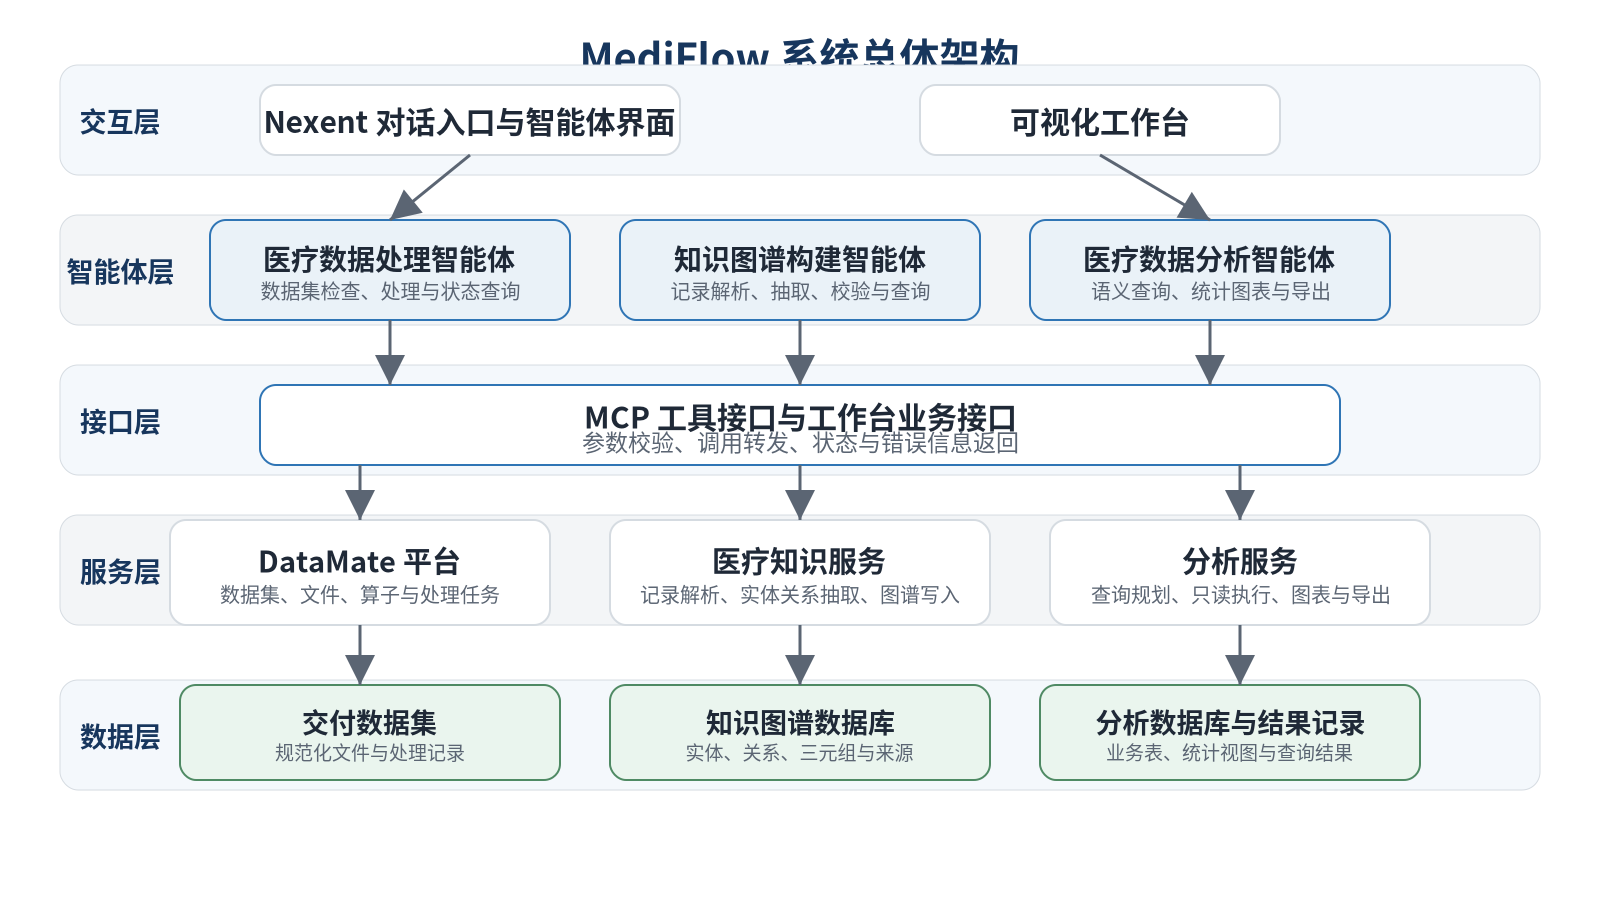
\includegraphics[width=0.98\textwidth]{figures/revision_architecture.png}
\caption{MediFlow 的分层架构与阶段数据对象}
\label{fig:architecture}
\end{figure}

DataMate 提供数据集、文件、算子和任务管理功能~\cite{datamate}。
Nexent 提供智能体配置、工具绑定、版本发布和对话执行功能~\cite{nexent,nexentdocs}。
项目使用 Model Context Protocol 连接 Nexent 与工具服务~\cite{mcpspec}，
在此基础上实现医疗格式路由、抽取校验、图谱持久化、查询安全和成果生成。
任务三还提供独立工作台入口，
它与 Nexent 查询工具共享图谱数据库和分析数据库，
用于集中呈现查询计划、关系图、统计图与成果下载。

\section{智能体工具调用机制}

智能体把用户任务转换为结构化工具调用，不直接执行文件处理、数据库写入或 SQL。图~\ref{fig:agent-call-chain} 展示一次调用的边界：Nexent 根据职责提示和工具说明识别任务类型，以工具名称和参数发起请求；FastMCP 将请求转交给 MediFlow 服务；服务按参数和数据状态选择处理流程，并把状态、产物标识和处理记录返回给智能体。

\begin{figure}[H]
\centering
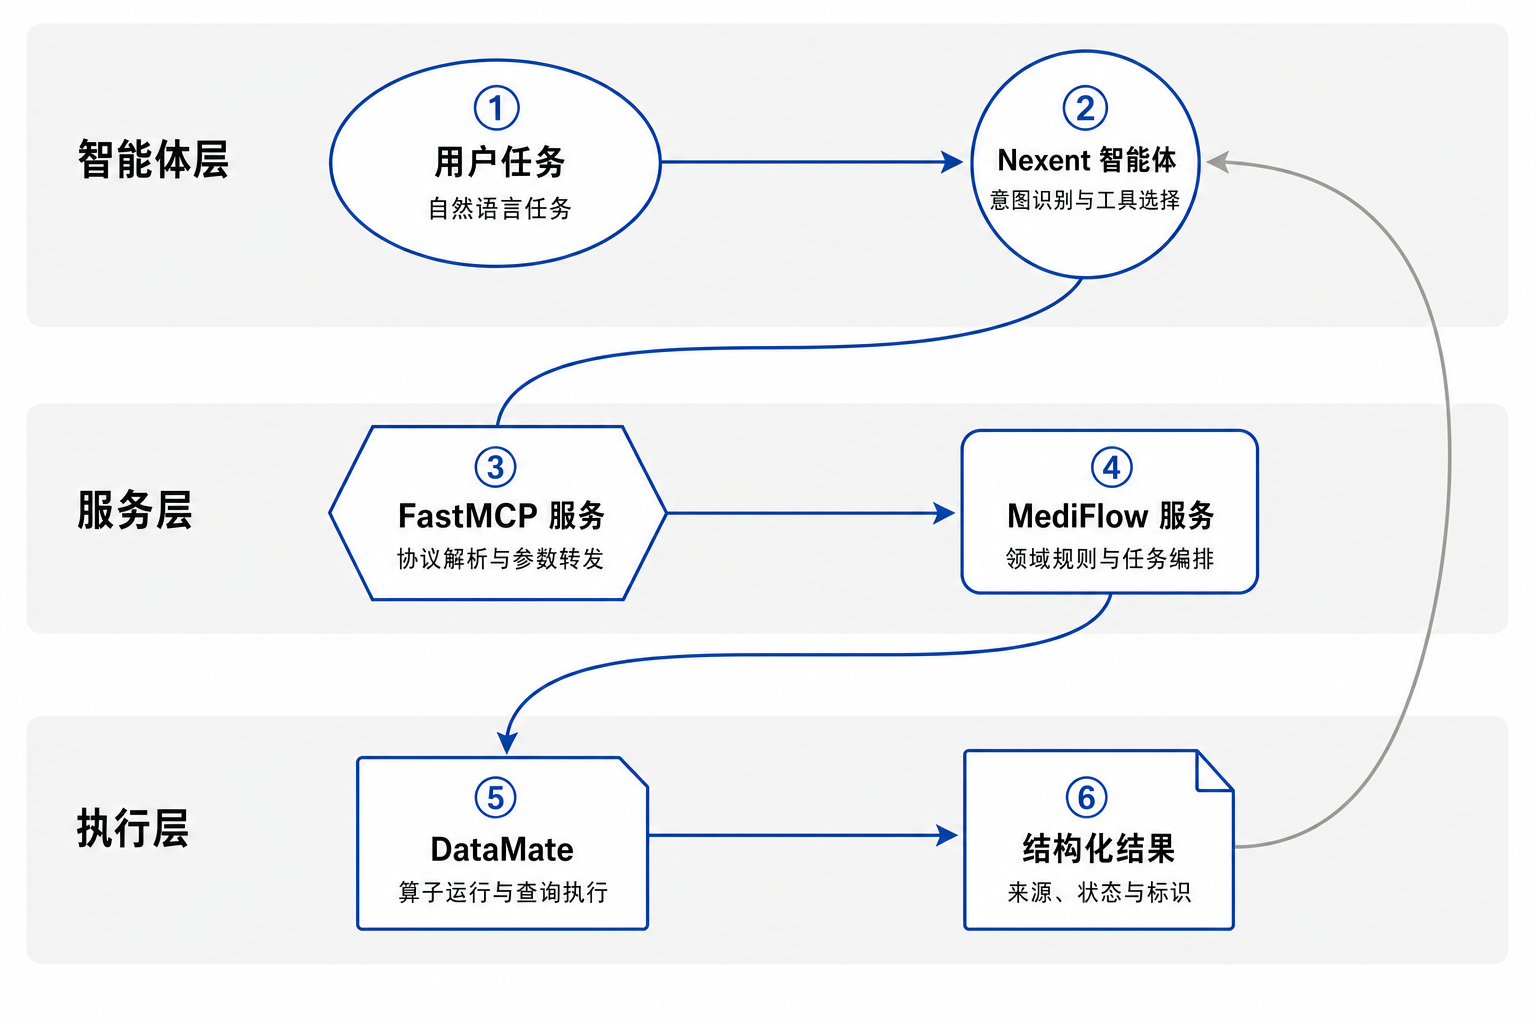
\includegraphics[width=0.96\textwidth]{figures/agent_call_chain_layered.png}
\caption{智能体单次调用的分层过程}
\label{fig:agent-call-chain}
\end{figure}

三个智能体使用不同的工具集合和职责规则。职责提示规定任务范围、工具调用顺序、参数来源和回复格式；约束提示规定只读边界、错误处理和禁止虚构结果；工具说明向模型提供接口名称、参数和返回字段。
模型据此选择任务级入口，
而不是直接决定每一个底层算子。
例如，任务一由智能体选择\texttt{run\_task1\_mixed\_cleaning}，
服务再按文件类型建立 DataMate 子任务和算子链。

工具返回的结构化状态决定后续动作。
小数据集完成后直接返回交付数据集，
大数据集返回运行标识并等待状态查询；
任务二返回抽取和入库状态，
任务三返回查询计划、数据行和分析标识。
工具调用失败时，智能体依据错误字段说明失败阶段和下一步，
实际产物以服务返回的状态和标识为准。

\begin{figure}[H]
\centering
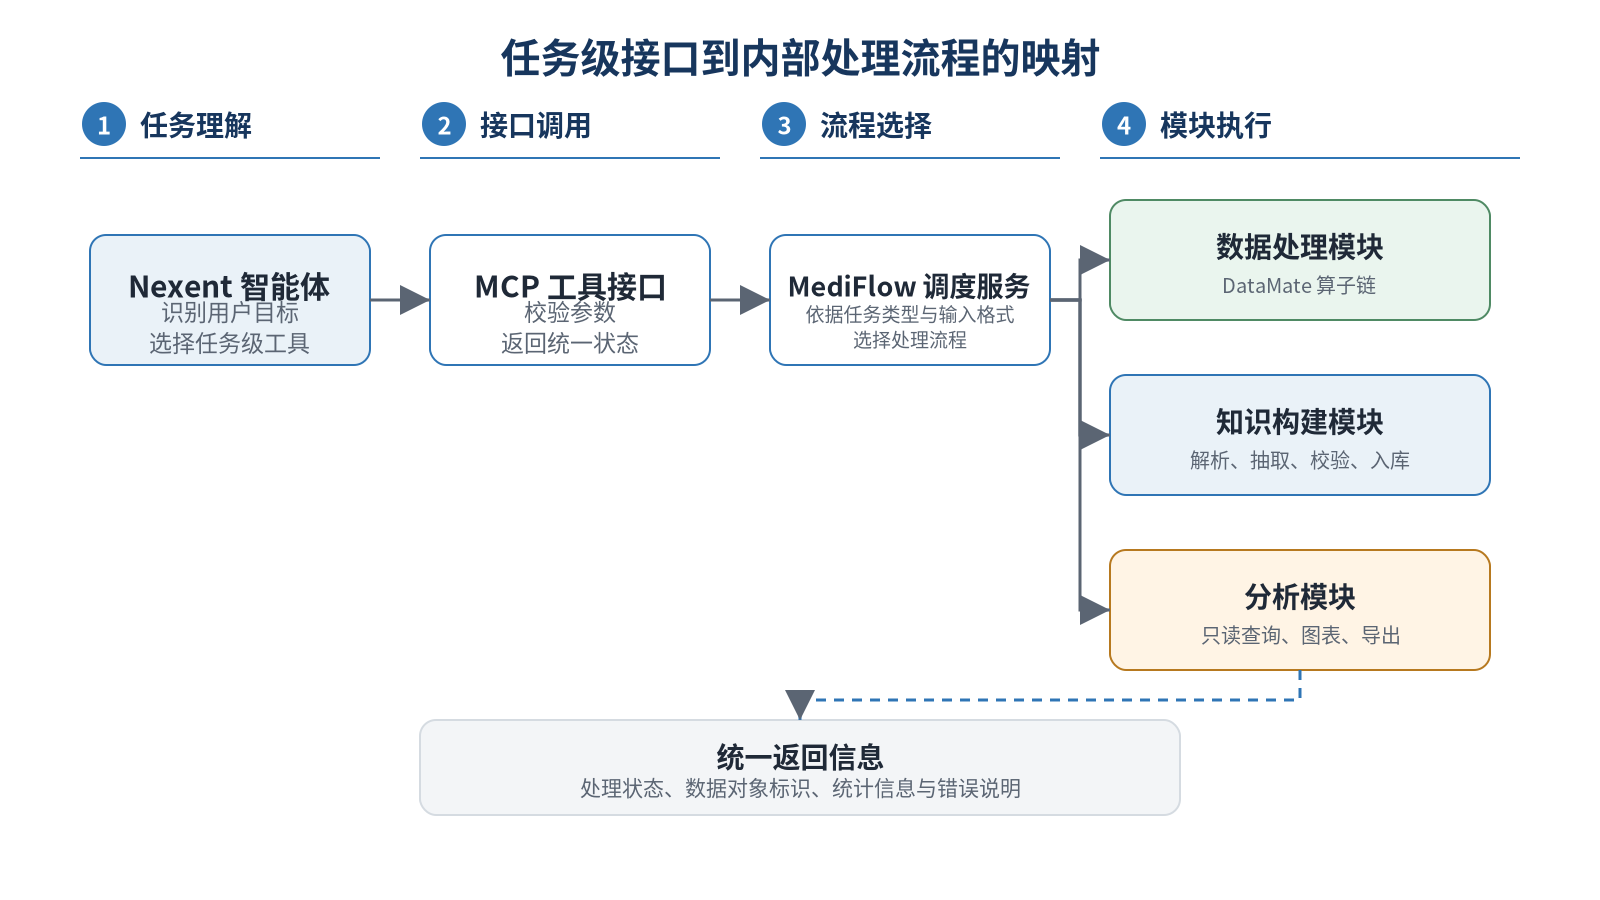
\includegraphics[width=0.96\textwidth]{figures/revision_task_mapping.png}
\caption{任务级工具到内部处理分支的映射}
\label{fig:task-interface-mapping}
\end{figure}

\subsection{DataMate 算子体系与执行边界}

DataMate 算子承担单步数据变换。项目算子采用 DataMate 的 Mapper 接口，由 \texttt{execute} 接收样本字典或文件记录，返回更新后的字段和处理记录；\texttt{metadata.yml} 保存注册信息。MediFlow 根据文件格式或抽取后端建立算子计划，DataMate 执行单步算子并返回结果；Nexent 只选择任务级 MCP 工具，不直接指定底层算子。

表~\ref{tab:operator-system} 归纳项目中的算子类别和执行边界。

\begin{table}[H]
\centering
\small
\caption{MediFlow 算子类别与执行边界}
\label{tab:operator-system}
\begin{tabularx}{\textwidth}{L{2.5cm}L{5.1cm}Y}
\toprule
\textbf{类别} & \textbf{代表算子} & \textbf{主要结果} \\
\midrule
通用清洗 &
EmojiCleaner、UrlRemover、WhitespaceNormalizer 等平台清洗算子 &
字符、链接、空白和文档噪声治理 \\
\addlinespace
医疗治理 &
MedicalTermNormalizer、MedicalTextQualityFilter、LLMNoiseFilter &
术语替换、质量筛选和噪声处理记录 \\
\addlinespace
结构保持 &
TableColumnCleaner、JsonFieldCleaner &
按字段清洗，保留表头、键名和嵌套层次 \\
\addlinespace
知识抽取 &
 MedicalEntityExtractor、MedicalRelationExtractor、MedicalTripleGenerator &
 实体关系抽取和三元组生成 \\
\addlinespace
记录组织 &
 MedicalRecordSplitter &
 按段落和句子边界拆分医疗记录，保留源文件与分段序号 \\
\addlinespace
统一输出 &
UnifiedJsonlExporter &
将多格式记录整理为任务二可读取的 JSONL \\
\bottomrule
\end{tabularx}
\end{table}

任务一在线流程直接创建 DataMate 清洗任务并轮询状态。
任务二的算子目录提供可注册的抽取资产，当前在线建图入口由
\texttt{run\_task2\_kg\_pipeline} 调用共享抽取服务，
再完成校验、入库和分析表刷新；两条路径共用实体关系模型和校验模块，
运行边界分别由 DataMate 任务和任务二领域服务负责。

图~\ref{fig:operator-execution} 将这条边界展开为一次完整调用：
智能体只选择任务级工具，服务再把参数映射为算子链或领域服务，
阶段产物统一回到带有状态和来源的结果记录。

\begin{figure}[H]
\centering
\begin{tikzpicture}[
  node distance=6mm and 7mm,
  main/.style={rectangle,draw=black!75,rounded corners=2pt,minimum width=3.0cm,
    minimum height=11mm,inner sep=3pt,align=center,font=\small,fill=blue!8},
  service/.style={rectangle,draw=black!75,rounded corners=2pt,minimum width=3.2cm,
    minimum height=11mm,inner sep=3pt,align=center,font=\small,fill=cyan!12},
  branch/.style={rectangle,draw=black!75,rounded corners=2pt,minimum width=3.2cm,
    minimum height=13mm,inner sep=3pt,align=center,font=\scriptsize},
  output/.style={rectangle,draw=black!75,rounded corners=2pt,minimum width=5.0cm,
    minimum height=10mm,inner sep=3pt,align=center,font=\small,fill=green!10},
  arrow/.style={-{Latex[length=1.8mm,width=1.1mm]},line width=0.65pt,
    draw=black!80,shorten <=2pt,shorten >=2pt},
  line/.style={line width=0.65pt,draw=black!80,shorten <=2pt,shorten >=2pt}
]
  \node[main] (agent) {Nexent 智能体\\任务理解与工具选择};
  \node[main,right=of agent] (mcp) {任务级 MCP 工具\\参数与状态边界};
  \node[service,right=of mcp] (service) {MediFlow 服务\\格式与后端映射};

  \node[service,below=9mm of service] (plan) {处理计划\\选择算子链或领域服务};
  \node[branch,fill=blue!8,below left=8mm and 6mm of plan] (task1)
    {任务一\\DataMate 清洗算子链};
  \node[branch,fill=blue!8,below=8mm of plan] (task2)
    {任务二\\抽取算子或共享服务};
  \node[branch,fill=gray!12,below right=8mm and 6mm of plan] (task3)
    {任务三\\只读分析查询服务};

  \node[output,below=8mm of task2] (output)
    {阶段产物与证据\\数据集、图谱事实、分析结果对象};

  \draw[arrow] (agent) -- (mcp);
  \draw[arrow] (mcp) -- (service);
  \draw[arrow] (service) -- (plan);

  \coordinate (branchpoint) at ($(plan.south)+(0,-3mm)$);
  \draw[line] (plan.south) -- (branchpoint);
  \draw[arrow] (branchpoint) -| (task1.north);
  \draw[arrow] (branchpoint) -- (task2.north);
  \draw[arrow] (branchpoint) -| (task3.north);

  \coordinate (outputpoint) at ($(output.north)+(0,3mm)$);
  \draw[line] (task1.south) |- (outputpoint);
  \draw[arrow] (task2.south) -- (output.north);
  \draw[line] (task3.south) |- (outputpoint);
\end{tikzpicture}

\caption{任务级工具到 DataMate 算子链的执行边界}
\label{fig:operator-execution}
\end{figure}

\section{智能体角色与工具配置}

项目按数据、知识和分析划分三个专业角色，
表~\ref{tab:agent-product-design} 从用户任务、执行逻辑和产物三个角度说明职责。Nexent 配置决定智能体可见的工具集合，MediFlow 服务负责参数校验和阶段内执行，DataMate 负责数据任务。
三个已发布角色覆盖赛题流程，自定义智能体也可复用其中的单项或组合工具。

\begin{table}[H]
\centering
\small
\caption{三个智能体的职责与工具边界}
\label{tab:agent-product-design}
\begin{tabularx}{\textwidth}{L{2.7cm}L{3.4cm}L{4.2cm}Y}
\toprule
\textbf{专业角色} & \textbf{用户任务} & \textbf{核心执行逻辑} & \textbf{主要产物} \\
\midrule
医疗数据处理 &
探查数据集、启动处理、查询进度、取得结果 &
识别五类文件，创建格式子数据集，运行 DataMate 算子链并汇聚结果 &
交付数据集、文件状态与处理报告 \\
\addlinespace
知识图谱生成与问答 &
从数据集建图、从文本抽取、查询疾病事实和关系 &
把文件解析为记录流，合并本地与模型抽取，校验后增量入库并刷新分析表 &
来源、实体、关系、三元组和疾病分析表 \\
\addlinespace
数据分析与可视化 &
查询疾病属性、统计关系分布、核对来源、导出分析成果 &
优先使用医疗语义模板规划查询，校验只读 SQL，组织回答、图表和报告 &
分析结果记录与 HTML、CSV、JSON 成果包 \\
\bottomrule
\end{tabularx}
\end{table}

\section{阶段数据与存储设计}

系统根据数据的使用方式设置三类存储。
DataMate 保存待处理文件、算子任务和交付数据集；
知识图谱 SQLite 库保存规范化实体关系及其来源；
分析 SQLite 库保存面向疾病查询的关系表和统计视图。
任务三执行过程中生成一条分析结果记录。表~\ref{tab:data-contract} 列出各层的实际结构。

\begin{table}[H]
\centering
\caption{核心存储与阶段数据对象}
\label{tab:data-contract}
\begin{tabularx}{\textwidth}{L{2.8cm}L{5.0cm}Y}
\toprule
\textbf{对象} & \textbf{主要结构} & \textbf{作用} \\
\midrule
DataMate 数据集 &
数据集标识、文件清单、算子实例、清洗任务、目标数据集 &
承载任务一输入、分格式处理和最终交付 \\
\addlinespace
知识图谱库 &
\texttt{kg\_sources}、\texttt{kg\_entities}、\texttt{kg\_aliases}、
\texttt{kg\_relations}、\texttt{kg\_triples}、\texttt{kg\_quality\_issues} &
保存实体关系、原文片段、来源和质量记录 \\
\addlinespace
分析数据库 &
\texttt{diseases}、\texttt{disease\_facts}、9 张疾病关系表、
统计表与统计视图 &
支持疾病属性查询、分布统计和图表生成 \\
\addlinespace
分析结果记录 &
分析标识、问题、查询计划、SQL、数据行、图表配置和来源信息 &
统一驱动文字回答、结果表、图表和成果导出 \\
\bottomrule
\end{tabularx}
\end{table}

知识图谱库适合维护规范化实体、关系和事实来源，
分析数据库则按关系类型把三元组转换为疾病与症状、药物、检查、科室等直接可查的业务表。
这种双库结构使任务二可以按事实粒度增量写入，
任务三可以使用简单、稳定的 SQL 完成聚合查询。

\section{跨阶段执行链路}

一次完整业务过程由以下六步组成：

\begin{enumerate}
  \item 用户在 DataMate 准备资料数据集，数据处理智能体先读取文件清单与格式分布；
  \item 任务一按格式建立子数据集，执行相应算子链，并登记新的交付数据集；
  \item 任务二按源文件轮转读取记录，避免处理上限集中落在单个文件；
  \item 抽取结果经实体位置、类型、关系引用和置信度校验后写入图谱事务；
  \item 新增三元组写入成功后刷新疾病事实表、九类关系表和统计视图；
  \item 任务三使用语义模板或经过约束的查询计划访问分析库，生成回答、数据表、图表和导出文件。
\end{enumerate}

这套流程允许单独运行任一任务。
已有公开医学资源可直接构成基础知识图谱，
新接入资料则沿任务一、任务二进入同一图谱，
任务三使用统一的数据口径展示已有知识与新增知识。

\section{结果校验与安全边界}

任务一在结果汇聚前重新解析 JSON、JSONL 和 CSV 产物，
PDF 分支分别保存上传、解析、下载和正文转换状态；
文件数超过 50 时转为后台任务并返回运行标识。
任务二只接收九类医疗实体和关系映射表中的关系，实体必须能在原文中定位。抽取结果先按可靠性等级分为高、中、低三级，再分别进入主图谱、候选记录或拦截记录；通用三元组转换函数的 0.7 参数是默认下限，在线级联入口显式保留候选，由持久化规则完成最终分流。
任务三只允许访问预先登记的 17 张表和视图，
SQL 必须为单条 \texttt{SELECT} 或 \texttt{WITH} 语句，
数据库连接启用只读与 \texttt{query\_only}，
单次最多执行 4 项查询、每项最多返回 200 行并设置 5 秒中止条件。
这些控制直接嵌入处理链和数据库访问层，
对 Nexent 入口与独立工作台采用同一执行规则。

\chapter{医疗数据处理智能体}

\section{数据输入与处理目标}

医疗数据处理智能体向用户提供数据集探查、文件上传、医疗内容处理和状态查询。
当前发布配置绑定 5 项工具，
覆盖文本上传、数据集检查、算子查询、混合处理和进度查询。
用户提交 DataMate 数据集名称或标识后，
服务解析为平台数据集标识，读取处于可处理状态的文件清单，
再按文件内容与扩展名确定处理分支。任务一的目标是登记可供知识抽取的交付数据集，并同时返回规范化文本、原有字段结构、文件级处理状态、质量记录和来源记录。

任务一接收 TXT、CSV、JSON、JSONL 和 PDF 五类输入，
其中 Markdown 按文本处理，TSV 按表格处理。
系统把文件识别、格式分组、医疗内容处理、DataMate 子数据集创建、
算子任务执行、结构恢复、质量检查和交付数据集登记组织为一条服务流程，
见图~\ref{fig:task1-pipeline}。

\begin{figure}[H]
\centering
\resizebox{0.98\textwidth}{!}{\begin{tikzpicture}[node distance=5mm and 5mm]
  \node[reportbox,minimum width=2.5cm] (source) {DataMate\\源数据集};
  \node[reportbox,right=of source,minimum width=2.7cm] (inspect) {文件探查\\格式分组};

  \node[reportbox,right=8mm of inspect,yshift=11mm,minimum width=4.1cm] (text)
    {TXT 与 PDF 文本\\清洗算子链};
  \node[reportbox,right=8mm of inspect,minimum width=4.1cm] (table)
    {CSV 表格\\保结构算子链};
  \node[reportbox,right=8mm of inspect,yshift=-11mm,minimum width=4.1cm] (object)
    {JSON 与 JSONL\\保结构算子链};

  \node[reportbox,right=8mm of table,minimum width=2.9cm] (collect) {质量检查\\结果汇聚};
  \node[reportdata,right=of collect] (result) {交付数据集};
  \node[reportbox,below=9mm of collect,minimum width=4.1cm] (status)
    {执行记录：文件状态、产物标识、质量摘要};

  \draw[reportarrow] (source.east) -- (inspect.west);
  \draw[reportarrow] (inspect.east) -- ++(4mm,0) |- (text.west);
  \draw[reportarrow] (inspect.east) -- (table.west);
  \draw[reportarrow] (inspect.east) -- ++(4mm,0) |- (object.west);

  % 三条格式分支先汇入质量检查左侧的合流点，避免与执行记录箭头重叠。
  \coordinate (qualitymerge) at ($(collect.west)+(-5mm,0)$);
  \draw[reportline] (text.east) -| (qualitymerge);
  \draw[reportline] (table.east) -- (qualitymerge);
  \draw[reportline] (object.east) -| (qualitymerge);
  \draw[reportarrow] (qualitymerge) -- (collect.west);
  \draw[reportarrow] (collect.east) -- (result.west);
  \draw[reportarrow] (collect.south) -- (status.north);
\end{tikzpicture}
}
\caption{医疗数据处理流程}
\label{fig:task1-pipeline}
\end{figure}

\section{任务探查与状态跟踪}

探查服务按 DataMate 文件记录读取文件名、类型和预览内容，
汇总五类格式的文件数，并把未支持文件保留在结果清单中。
Nexent 根据用户表达选择“查看数据集”“启动处理”或“查询运行状态”；
进入处理后，具体算子组合由服务端格式映射表决定。
同一批文件因此只产生一份任务级计划，
计划中列出每个格式分组、所用算子链、临时数据集和目标文件形式。

同步处理适用于不超过 50 个文件的数据集。
文件数更大时服务建立后台运行记录并立即返回运行标识，
状态查询依次给出排队、运行、成功或失败，
使长任务不占用一次对话请求。

任务一智能体按用户表达区分三类动作：
查看数据集时调用\path{inspect_dataset}，
执行混合格式清洗时调用\path{run_task1_mixed_cleaning}，
查询后台进度时调用\path{get_task1_mixed_cleaning_status}。
用户直接提供原始文本时，
智能体先调用\path{upload_text_to_datamate}取得真实数据集标识，
再把该标识传给数据集探查和清洗工具。

智能体只负责选择任务级工具并传递真实标识。
工具服务读取文件清单后，
由格式映射表决定文本、表格、结构化文件和 PDF 的处理链，
因此模型不会绕过结构校验直接指定算子。
工具返回\texttt{run\_id}时，
智能体继续查询状态；返回错误时，
回答保留错误阶段和已完成分组，部分产物仍按服务状态标记。

\section{文本治理与结构保持}

五类格式共享字符级基础治理，
包括表情符号、URL、乱码、不可见字符、全半角、繁简体、HTML 标记和空白规范。
文本分支继续执行长度、重复短语、特殊字符和重复文件过滤，
再进行医疗术语与缩写规范、语义噪声处理。
结构化分支只清理文本字段，并在结果汇聚阶段恢复原有结构。

医疗术语规范由 MedicalTermNormalizer 算子执行，
采用词典优先、LLM 兜底的混合策略。
词典数据来自瑞金糖尿病研究中的医学术语和通用医学缩写库，
共 114 条映射（\repoPath{operators/medical\_term\_normalizer/term\_kb.db}），
覆盖“T2DM→2型糖尿病”“AMI→急性心肌梗死”等高频缩写。
词典命中后直接替换，未覆盖的缩写交由 LLM 补充处理，
LLM 调用失败时退回词典结果。
算子返回每条替换的原文、替换后文本和出现次数。

语义噪声处理由 LLMNoiseFilter 算子执行。
该名称沿用算子注册名，当前实现读取 SQLite 规则库
（\repoPath{operators/llm\_noise\_filter/noise\_kb.db}）中通过审核并启用的规则。
规则素材来源于 cMedQA2 中文医疗问答社区数据，
覆盖广告营销、联系方式、系统导出标记、测试数据标记、网页尾部信息和 URL 链接等噪声类型。
算子将文本逐条匹配规则，命中段落按规则指定的范围（行、句子或文本块）移除，
并记录拦截类型、匹配规则和移除内容，形成文件级质量记录。
规则库独立于算子代码，新增规则只需更新数据库，
无需修改算子逻辑或重新注册。

固定规则无法提前列出病历中不断出现的闲聊和交接文字。
系统因此记录教师清洗前后的差异，并从历史差异中寻找重复片段。
同一片段至少出现 3 次、类别位于安全清单、且不含疾病、症状、药物或医学数值时，
系统才将它写入规则库。后续文件直接复用该规则，不再重复调用模型。
这项机制学习的是经过确认的重复噪声模板，不把未见表达误报为已经掌握的语义能力。

服务只报告算子实际返回的处理项，不根据提示词推测清洗效果。字符变化、解析错误、空文本、重复内容和结构复核共同组成文件级质量摘要。

服务端在 \texttt{mcp\_server/task1/chains.py} 中维护格式到算子链的映射。
文本和 PDF 复用基础清洗、文档质量检查、MedicalTermNormalizer 与 LLMNoiseFilter；
CSV 进入 TableColumnCleaner，JSON 和 JSONL 进入 JsonFieldCleaner。
PDF 先由 MinerU 转换为 TXT，再复用文本链，
因此 PDF 解析属于输入适配，医疗内容治理仍由 DataMate 算子完成。

\begin{table}[H]
\centering
\caption{医疗内容治理与结构处理方式}
\label{tab:task1-format-routing}
\begin{tabularx}{\textwidth}{L{1.7cm}L{5.2cm}Y}
\toprule
\textbf{格式} & \textbf{处理单元与算子组合} & \textbf{交付结构} \\
\midrule
TXT &
整篇或分段文本；基础治理、文档质量过滤、医疗术语与缩写规范、语义噪声处理 &
合并分段并输出 TXT \\
\addlinespace
CSV &
保留表头与行列位置；基础清理后执行表格列清理 &
保持列名、列顺序和 CSV 格式 \\
\addlinespace
JSON &
递归处理对象与数组中的文本值；基础清理后执行 JSON 字段清理 &
保持键名、嵌套层次和 JSON 对象结构 \\
\addlinespace
JSONL &
逐行解析对象并清理文本字段 &
保持一行一条 JSON 记录 \\
\addlinespace
PDF &
MinerU 提取正文并转换为文本，再执行 TXT 处理链 &
以同名 TXT 作为交付文件 \\
\bottomrule
\end{tabularx}
\end{table}

图~\ref{fig:task1-contract} 把五类输入的处理单元、格式专用步骤和交付结构展开到字段层面。
公共交付步骤负责结构恢复、重新解析检查和文件状态登记，
因此任务二能够沿同一数据集标识读取清洗结果。

\begin{figure}[H]
\centering
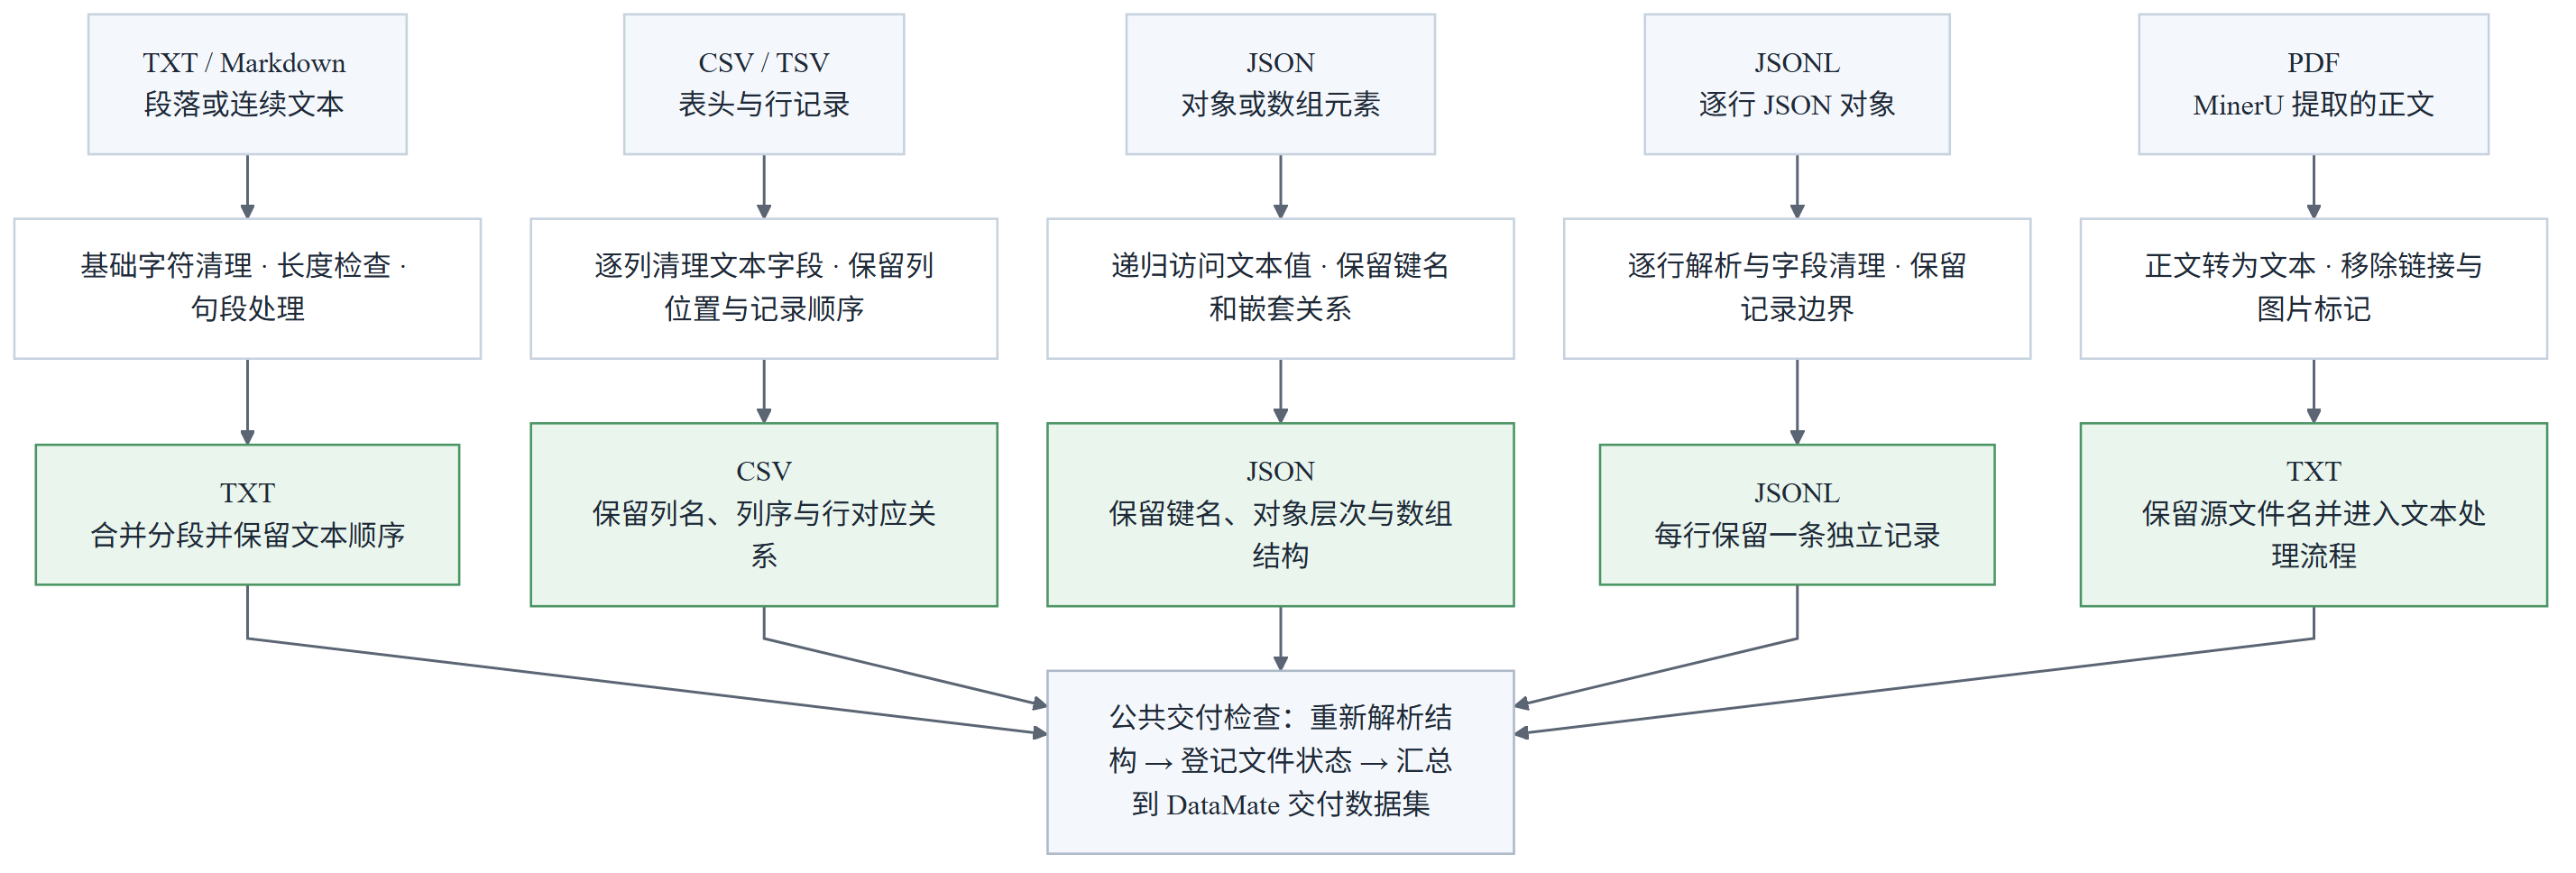
\includegraphics[width=0.98\textwidth]{figures/mermaid_format_structure.png}
\caption{五类输入的格式专用处理与结构保持结果}
\label{fig:task1-contract}
\end{figure}

文本算子可能产生带序号的分段文件，
汇聚服务按原文件名和分段序号重新合并；
JSON 与 JSONL 结果恢复扩展名后再次解析，
CSV 结果重新读取表头。
完成结构检查的文件进入最终数据集，
任务二可以继续按字段读取结构化资料。

\section{失败隔离与结果交付}

混合编排服务先按五类格式建立临时子数据集，
再为每个非空分组创建 DataMate 清洗任务。
任务返回目标数据集后，
服务读取实际产物并完成分段合并、扩展名恢复和结构检查。
各分组采用独立任务，某一格式失败时仍可保留其他分组的完成结果和文件状态。

最终交付数据集由各格式分组的合格产物重新汇聚而成。
服务将这些产物登记到一个 DataMate 数据集中，
同时返回源数据集、格式分组、算子方案、子任务、目标数据集、
文件级报告、处理性能和治理元数据。
这些字段共同说明“处理了哪些文件、经过哪条链、产物存放在哪里”，
并为任务二提供可直接解析的数据集标识。

\section{PDF 文档适配}

PDF 是任务一的文档输入适配分支，不改变后续医疗内容治理逻辑。
项目通过 MinerU 接口完成版面解析和正文提取~\cite{mineru2024,minerurepo}，
客户端负责文件上传、任务轮询和结果下载。
服务从解析产物中选择正文 Markdown，
去除版式标记后生成 TXT 文件，
再进入与普通文本相同的 DataMate 算子链。

当前适配器单次处理一份 PDF，
上传前检查文件有效性、10\,MB 大小限制和 20 页页数限制，
并为上传、轮询、结果下载、正文缺失和超时分别返回状态。
PDF 结果明确标记为文本交付，
其他格式继续保持源格式。
正文解析结果通过 Markdown 语法树提取段落与表格文字，
链接和图片标记在进入文本清洗链前被移除。

\section{交付数据与质量记录}

\begin{table}[H]
\centering
\caption{医疗数据处理智能体的交付内容}
\label{tab:task1-delivery}
\begin{tabularx}{\textwidth}{L{3.2cm}L{4.3cm}Y}
\toprule
\textbf{交付项} & \textbf{主要内容} & \textbf{后续用途} \\
\midrule
交付数据集 &
清洗后的 TXT、CSV、JSON、JSONL 文件及 PDF 转换文本 &
作为任务二知识抽取输入 \\
\addlinespace
分组任务结果 &
各格式子数据集、DataMate 任务、算子方案和目标数据集 &
查看平台任务与分支执行状态 \\
\addlinespace
文件处理记录 &
源文件、识别格式、输出文件、完成状态和处理信息 &
定位单个文件的处理结果 \\
\addlinespace
质量摘要 &
文件数、记录数、术语替换、噪声处理、格式检查和结构恢复结果 &
核对交付数据是否满足后续读取要求 \\
\bottomrule
\end{tabularx}
\end{table}

任务一把文件级算子执行组织为数据集级治理交付：
用户在 Nexent 中发起一次任务，
DataMate 承载多个格式子任务，
项目服务负责结构保持与结果汇聚，
最终得到可直接进入知识抽取的数据集入口和可核验的处理记录。

\chapter{医疗知识构建与问答}

任务二以任务一产出的清洗数据集为输入，
经过记录解析、实体关系抽取、校验去重和图谱持久化，
生成可查询的医疗知识图谱，并同步刷新面向分析查询的派生表。
智能体同时绑定建图工具和查询工具，
用户可以在一次对话中完成从数据集到图谱查询的完整流程。

\section{参考知识与增量数据接入}

图谱的基础知识层由两个外部数据源和一个内部质检参考共同构成，
通过 \repoPath{kg/build\_kg\_v2.py} 统一写入 SQLite。

\textbf{QASystemOnMedicalKG（图谱主体）。}
这是一个开源中文医学知识图谱项目~\cite{qasystemkg}，
其核心文件 \texttt{medical.json} 以 JSONL 格式收录了 14\,408 种疾病的结构化信息，
每种疾病携带症状、药物、检查、科室、并发症、病因、预防等字段。
构建脚本逐行解析后，按字段到关系的映射表
（如 \texttt{symptom}→临床表现、\texttt{recommand\_drug}→药物治疗、
\texttt{check}→检查、\texttt{cure\_department}→就诊科室）
将每条字段值拆分为三元组写入图谱，
贡献 420\,221 条三元组。
写入过程中对症状字段执行质量检查：
以从 CMeEE 标注数据中提取的症状词汇表为参照，
筛除不包含典型症状字眼且不在词汇表中的条目
（如人名、乱码、数据污染），
被筛除的条目写入质量记录表而不进入图谱。

\textbf{CMeIE 标注数据（关系补充）。}
CMeIE 是 CBLUE 基准中的中文医学信息抽取数据集~\cite{cblue2022}，
包含 14\,339 条已标注实体和关系的句子。
构建脚本将标注的实体对和关系类型
通过 \texttt{CMEIE\_RELATION\_MAP} 映射为项目的 15 类标准关系后入库，
贡献 25\,046 条三元组。
此外，CMeIE 定义的 43 种关系类型和实体类型体系
也是后续抽取校验模块中类型合法性的判断依据
（\repoPath{core/medical\_extraction\_validation.py} 的 \texttt{ENTITY\_TYPES} 和 \texttt{CMEIE\_RELATION\_TYPES}）。

\textbf{CMeEE 标注数据（质检词典）。}
CMeEE 同样是 CBLUE 的标注数据，用于实体识别评测。
在离线构建阶段，构建脚本从中提取全部已标注的症状实体，
形成一份“确认是症状”的词汇表，
用于过滤 \texttt{medical.json} 中质量存疑的症状字段。
CMeEE 本身不直接导入图谱，
而是作为质检参考标准参与基础知识层的质量把关。

三者的分工是：
QASystemOnMedicalKG 提供覆盖面，CMeIE 提供标注精度，
CMeEE 提供质检依据。
基础构建程序还定义了 15 类标准关系，
以关系代码和中文显示名分开保存，
使不同数据来源中的“临床表现”“相关症状”等表达归并到统一查询口径。

基础知识层构建完成后，
任务一交付数据集进入任务二处理流程时，
每次处理都注册独立来源，
新增事实沿用同一套实体、关系和三元组表结构，
增量数据与基础知识共用同一查询和分析入口。当前在线实例中，
增量管道累计贡献 553 条三元组，
作为独立来源（DataMate 增量）与基础知识共存于同一统计口径。

\section{统一医疗记录解析}

任务二处理流程的第一步是将 DataMate 数据集中的清洗后文件转换为统一的记录流。
共享解析模块按文件扩展名和内容类型分派处理：
TXT 以空段落切分，单段超过 1\,200 字符时按句号边界继续拆分；
CSV 经 \texttt{csv.DictReader} 逐行序列化，保留列名作为字段键；
JSON 数组逐项生成记录，对象整体作为一条；
JSONL 按非空行逐条解析。
每条记录统一携带 \texttt{record\_id}、
\texttt{source\_file}、\texttt{source\_format} 和原始字段；
结构化记录原本带有 \texttt{record\_id} 或 \texttt{id} 时，另存为
\texttt{source\_record\_id}，否则使用源文件名加行号或分段号生成稳定记录号，
确保下游抽取模块无需区分原文件的物理格式。

当用户通过 \texttt{max\_records} 参数限制单次处理量时，
选择模块采用跨文件轮转抽样：按源文件分桶后轮流从各桶取一条，
使处理额度在各文件之间均匀分配。
例如 5 个文件各 100 条记录、限制 50 条时，
每个文件贡献 10 条。

\begin{figure}[H]
\centering
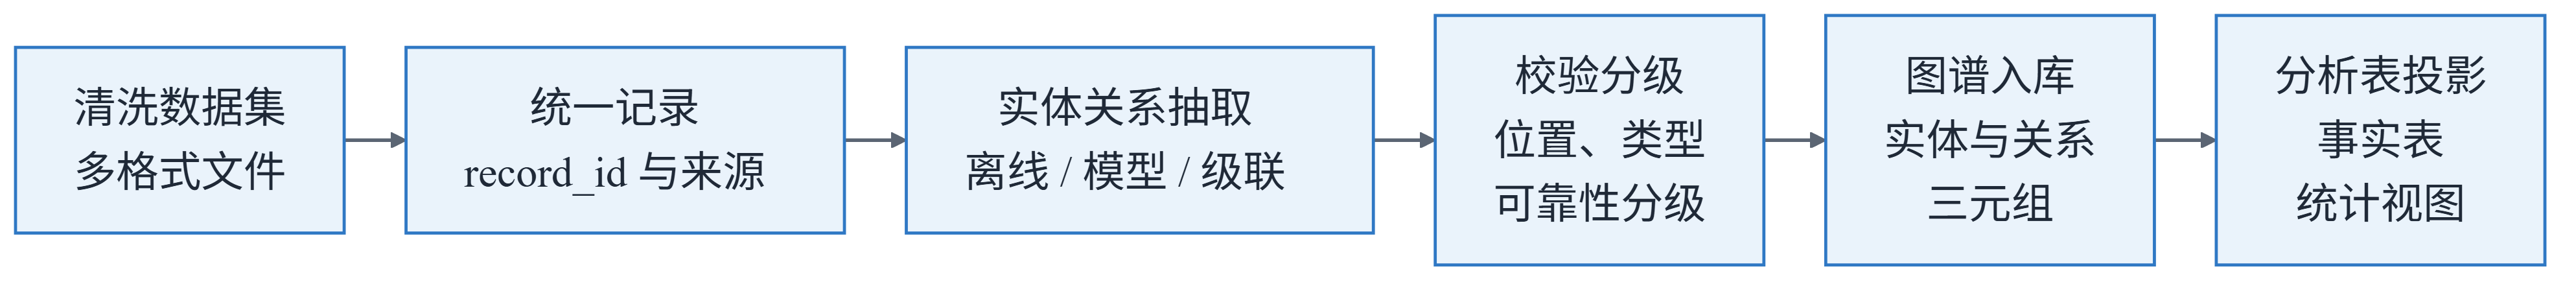
\includegraphics[width=0.98\textwidth]{figures/mermaid_kg_pipeline.png}
\caption{清洗数据集到知识图谱和分析表的处理流程}
\label{fig:task2-pipeline}
\end{figure}

\section{实体关系级联抽取}

统一抽取服务提供三种可切换的后端。

任务二的 DataMate 算子把记录处理拆成可注册的单步处理。
表~\ref{tab:task2-operators} 给出算子接口与在线建图服务的对应关系。

\begin{table}[H]
\centering
\small
\caption{任务二算子接口与处理结果}
\label{tab:task2-operators}
\begin{tabularx}{\textwidth}{L{3.1cm}L{4.8cm}Y}
\toprule
\textbf{算子} & \textbf{输入与处理} & \textbf{输出字段} \\
\midrule
\makecell[l]{MedicalEntity\\Extractor} &
读取记录文本，按离线、模型或混合后端识别九类医疗实体 &
\texttt{entities}、后端标识和抽取耗时 \\
\addlinespace
\makecell[l]{MedicalRelation\\Extractor} &
结合实体结果抽取疾病与其他实体之间的关系 &
\texttt{relations}、后端标识和抽取耗时 \\
\addlinespace
\makecell[l]{MedicalTriple\\Generator} &
将实体关系转换为三元组，并按可靠性等级分流 &
\texttt{triples}、入库数量和质量记录 \\
\addlinespace
\makecell[l]{MedicalText\\QualityFilter} &
检查医疗文本长度、特殊字符比例和重复内容 &
质量状态、过滤原因和处理统计 \\
\bottomrule
\end{tabularx}
\end{table}

上述算子以 \texttt{operators/*/process.py} 和 \texttt{metadata.yml} 作为可部署资产。
在线建图入口读取 DataMate 数据集后，
由 \texttt{core/medical\_extraction\_service.py} 选择抽取后端，
再由任务二服务完成校验、事务写入和分析库刷新。
算子接口和在线服务共享抽取模型与校验逻辑，
调用入口分别面向 DataMate 任务和数据集级 MCP 工具。

对于用户在 Nexent 中直接给出或要求生成的一段医疗文本，智能体调用统一文本抽取工具
（\texttt{extract\allowbreak\_medical\allowbreak\_knowledge\allowbreak\_from\allowbreak\_text}）。
该入口只运行一次抽取链，同时返回
\texttt{entities}、\texttt{relations}、\texttt{triples}、
\texttt{cascade}、\texttt{performance} 和 \texttt{extraction\_errors}。
返回空数组表示该段文字未识别到相应事实，仍属于结构完整的成功结果；
三个拆分入口保留用于兼容单项调用，但智能体不再把同一文本重复抽取三次。
自拟病历在调用前移除引号并整理为一个纯文本参数，避免对话平台把病历中的引号误判为调用语法边界。

\subsection{离线词典规则抽取}

离线抽取模块实现了不依赖外部模型的抽取链。

\textbf{实体识别}的执行过程为：
第一，加载独立维护的医学词典 \texttt{entity\_lexicon.json}，
当前资产包含约 3.17 万条术语，词条由 CMeEE-V2 和 CMeIE 训练数据整理生成；
运行时再与已有图谱实体合并，统一映射到 CMeEE 的实体类型；
第二，长词优先匹配：先匹配“2型糖尿病”再匹配“糖尿病”，
已占用的字符区间不再被短词覆盖；
第三，过滤停用词（“患者”“医生”“治疗”等通用词）、
纯数字串、长度小于 2 或大于 32 的字符串；
第四，为每个命中位置截取前后各 20 个字符作为原文片段。

\textbf{关系抽取}以疾病为中心，但不再把句内共现直接视为事实。
模块先在同一句或受限文本窗口内定位疾病与其他实体，
优先复用图谱和 CMeIE 资产中已经出现过的主客体关系；
没有已知关系时，必须同时满足实体类型约束和关系触发词，
例如“表现为”支持临床表现，“位于、累及”支持发病部位，
“由于、导致”支持病因，“给予、服用”支持药物治疗。
仅有实体共现、没有对应触发证据的候选不会直接形成关系。
对于 CMeIE 常见的“疾病@正文”结构，标题疾病会在同一分段的后续句中继承，
使检查、部位和病因等关系仍有明确主语；遇到新的疾病标题时立即切换归属。
普通病历还识别“初步诊断、入院诊断、出院诊断”等明确诊断句：
诊断后的三句、360 个字符以内，给药、实施治疗和并发症枚举可以继承最近的首个诊断疾病；
跨空段或遇到新的诊断句即停止继承。该窗口只解决“诊断在前一句、处理在后一句”的病历写法，
不把整段任意共现实体相互连接。
最后，\texttt{NEGATION\_RE} 检查“无”“未见”“否认”“排除”等否定表达，
命中否定范围的实体不生成关系。

\subsection{模型补充抽取}

\texttt{core/medical\_ner.py} 和 \texttt{core/medical\_re.py}
将医疗记录组织为结构化抽取请求，
要求模型返回实体（文本、类型缩写、起止位置）和关系（头尾实体、关系类型），
均为 JSON 数组格式。
模型返回的结果随后经过与离线方式相同的校验和去重管道。

\subsection{离线优先级联抽取}

\texttt{hybrid}（混合方式）采用离线优先的级联流程，
先扫描全文，再根据句子覆盖情况和候选可靠性决定模型的使用范围。
离线方式和混合方式的第一阶段调用同一套词典、关系规则和质量门禁。
句子覆盖情况由句内已识别实体、关系以及医疗提示词共同判断：
若存在未参与关系的实体、关系类型缺失或因果、部位等提示词未得到对应关系，
该句进入待补充集合；没有这些情况的句子直接进入统一校验。
高、中可靠离线候选直接保留；低可靠实体进入 LLM 复核；
低可靠关系只放行两类窄候选：历史分组精确率达到路由条件且带原文触发词的候选，
以及“明确给药句、明确诊断后续句”产生并已通过确定性证据检查的候选；
旧的泛句内共现和全文上下文候选仍被门禁拦截；
离线链路未覆盖但包含医疗提示词的句子进入模型补充，
模型只能返回原文直接支持的实体和关系。
图~\ref{fig:task2-cascade} 展示了这条处理路径。

\begin{figure}[H]
\centering
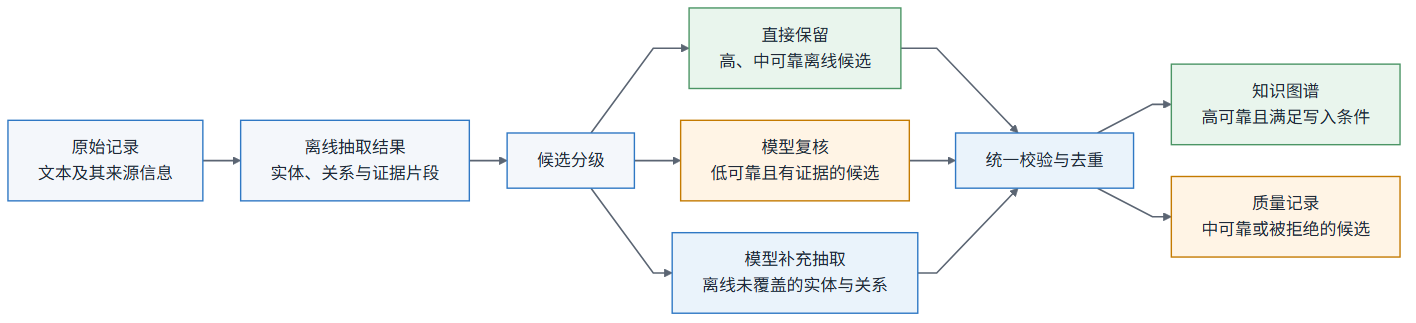
\includegraphics[width=0.98\textwidth]{figures/mermaid_cascade.png}
\caption{离线优先的实体关系级联抽取流程}
\label{fig:task2-cascade}
\end{figure}

级联流程由任务二服务负责编排。服务根据句子内实体和关系覆盖情况筛选待补充句，并限制一次模型补充的句子数量；模型调用只返回原文直接支持的实体和关系。模型补漏实体与复核恢复的低可靠离线实体共用同一套规范化门禁，统一检查原文边界、完整词形、实体类型、否定范围和噪声片段。实体的起止位置必须与原文切片逐字相等，例如原文只有“胸痛”时，“胸痛（术后）”不能通过；新增关系还必须通过端点存在性、关系类型和触发词证据校验。高分且属于已校准安全类型的候选可以直接进入合并，其余候选再与低可靠离线候选一起复核。
复核通过的新增事实标记为高可靠，
抽取方式字段写入 \texttt{llm\allowbreak\_gap\allowbreak\_verified}。
其两个端点也必须通过实体校验；
缺失、拒绝或不确定的决定不会新增事实。

批量处理分两阶段完成：
第一阶段逐条执行离线抽取，并为每条记录加上独立候选范围；
第二阶段只对存在待补充句的记录并发调用模型补充，
每批最多使用 4 个工作线程，单条调用超时后保留该记录的离线结果。
待补充关系、低可靠离线关系、待补充实体和低可靠离线实体按顺序进入复核队列；每一层都按记录轮转抽取候选，避免前部记录占满额度。
队列上限为 256 条；随后调用 \path{review_candidates()} 统一处理。
合并阶段以记录标识限定候选范围，避免批量处理时将其他记录的复核结果错误关联到当前记录。
模型调用失败时，服务保留已经通过离线质量门禁的实体、关系和三元组，
并在处理结果记录的 \texttt{llm\_error} 字段中返回错误信息。
因此，\texttt{hybrid} 在保留离线可复现结果的同时，
只把有原文依据的补充事实交给后续入库流程。

\subsection{基于可靠性分级的事实持久化}

系统从 \texttt{reliability\_profile.json} 读取按处理阶段、抽取方法和实体或关系类型划分的验证结果，
将候选标记为高、中、低三级。配置中的分组精确率用于入库决策，
表示同组方法的历史可靠性，不表示单条事实的概率。

对离线候选，分组可靠性分按
\[
  p_g=\frac{TP_g}{N_g},\qquad
  g=(s,m,c)
\]
计算，其中 (s)、(m)、(c) 分别表示处理阶段、抽取方法和实体或关系类型，
\(N_g\) 是验证集中该组输出数量，\(TP_g\) 是严格命中的数量。
因此，同为“词典精确匹配+疾病”的多个实体会显示相同分数，这是按组校准的结果，不是程序把每条事实都判断成同一概率。
低可靠候选经模型明确接受后，抽取方式改为
\texttt{llm\_review\_verified}，可靠等级提升为高，界面分数改用本次模型裁决返回值；
该值仍是复核信号，不应解释为临床风险概率。

\begin{table}[H]
\centering
\caption{任务二候选事实的可靠性分级}
\label{tab:reliability-tiers}
\begin{tabularx}{0.82\textwidth}{L{2.6cm}L{3.4cm}Y}
\toprule
\textbf{等级} & \textbf{处理方式} & \textbf{写入结果} \\
\midrule
高 & 通过入库校验 & 写入 \texttt{kg\_triples}，保留来源标识、原文片段和抽取方式 \\
中 & 保留为候选 & 写入 \texttt{kg\_quality\_issues}，标记为 \texttt{candidate\_fact} \\
低 & 不进入主图谱 & 写入 \texttt{kg\_quality\_issues}，标记为 \texttt{rejected\_fact} \\
\bottomrule
\end{tabularx}
\end{table}

持久化层遇到缺失的可靠性标记时，将 LLM 结果按中等级处理，
其他来源按低等级处理。这样，只有明确归入高等级的事实进入主图谱，
中、低等级候选都保留在质量记录中，供复核和统计使用。

\subsection{知识构建与问答路由}

知识图谱生成与问答智能体根据用户目标选择不同工具入口。
用户要求处理数据集或重新建图时调用\path{run_task2_kg_pipeline}；
用户给出或要求生成单段医疗文本时调用\path{extract_medical_knowledge_from_text}，一次取得实体、关系、三元组和性能统计；
用户询问疾病属性时调用\path{query_disease_analytics}；
用户要求查看实体关系时调用\path{query_knowledge_graph}；
用户询问已登记来源时调用\path{get_medical_data_sources}。
这些工具共享同一套来源、实体和关系数据，
问答阶段读取的是建图阶段已经提交的事实。

建图工具和任务二服务默认使用 \texttt{hybrid} 后端，
先执行离线全量扫描，再按级联规则调用模型；
需要完全可复现的批量导入时，可以显式指定 \texttt{offline}。
智能体根据工具返回的\texttt{status}、来源文件摘要、生成三元组数量、
入库数量和分析库刷新状态组织回答；
部分记录失败或分析库未刷新时，
回答保留对应状态，并将候选抽取结果与已入库事实分别展示。

\section{实体关系校验与入库}

抽取产生的候选依次经过类型检查、字段归一化、可靠性分级与去重，
再由持久化服务完成数据库去重和写入。前四项检查由
\path{core/medical_extraction_validation.py} 负责，
持久化服务由 \path{mcp_server/kg/persistence.py} 执行最终写入。

\textbf{第一道：类型校验。}
实体类型只接受 9 类（疾病、症状、药物、设备、治疗、身体部位、检查、微生物、科室），
通过 \texttt{ENTITY\_TYPE\_ALIASES} 将中文名、英文名统一映射为内部缩写；
关系类型只接受 CMeIE 标准集中的 43 种，
通过 \texttt{RELATION\_ALIASES} 将“症状”“科室”等常见简称映射为标准名。
实体文本必须在原始记录中能够定位；模型结果给出的起止位置还必须满足
\texttt{text[start:end+1] == entity.text}，位置缺失时只接受原文中唯一的精确出现，
关系中的头尾实体名必须同时出现在原文中。

\textbf{第二道：归一化。}
抽取侧将模型返回的各种写法统一为内部代码
（实体类型“症状”→\texttt{sym}，关系别名“症状”→“临床表现”）；
持久化侧（\path{mcp_server/kg/normalization.py}）再映射为英文关系代码和中文展示名
（“临床表现”→\texttt{has\_symptom}，展示名“临床表现”；
“药物治疗”→\texttt{treated\_by\_drug}，展示名“药物治疗”）。
两层归一化确保离线词典、模型和混合三种抽取方式产出的字段落在同一值域。

\textbf{第三道：可靠性分级与去重。}
实体在校验函数内按出现位置和类型去重，
关系按主语、谓词和宾语去重；
三元组转换步骤再次按同一组合去重，并保留抽取置信度和可靠性等级。通用转换函数默认使用 0.7 的置信度下限；在线级联入口显式保留候选，最终是否进入主图谱由高、中、低三级持久化规则决定。0.7 阈值承担通用转换过滤，三级可靠性承担最终持久化分流。

\textbf{第四道：数据库去重与写入。}
持久化服务按记录逐条写入：先按名称和类型保持实体唯一，
再确保关系类型唯一，最后按主语、关系、宾语、来源标识和原文片段的组合写入三元组。
同一名称在不同实体类型中可以分别保留，
同一事实来自不同文件时各自保留独立来源标识和原文片段。
三元组同时保存 \texttt{source\_file} 和 \texttt{source\_record\_id}，
查询结果可返回来源数据集、文件、记录号、原文证据、抽取方式和可靠等级。

整个抽取和入库过程由任务二服务统一编排。
每条记录独立处理。某条记录的抽取失败不影响其他记录，
某条三元组的写入失败也不回滚已成功入库的部分。
循环结束后统计实体数、关系数、生成三元组数和实际入库数，
并计算平均抽取时延和吞吐量。

\section{图谱事实的分析投影}

图谱写入完成后，分析刷新服务按三元组中的关系类型，
将规范化事实写入面向查询的派生业务表；服务将这一步记为“分析表刷新”。
\texttt{diseases} 保存疾病主表，
\texttt{disease\_facts} 保存全部疾病事实；
症状、药物、科室、并发症、检查、治疗、病因、预防和易感人群
分别进入 9 张关系表。
\texttt{entity\_stats} 与 \texttt{relation\_stats} 保存统计结果，
五个视图提供实体类型、关系类型、高频症状、科室疾病和药物疾病分布。

刷新只在图谱事务提交成功且存在新增三元组时执行，
避免分析表早于图谱更新，或在没有新增事实时重复刷新。
图谱库承担规范化事实和来源追溯，
分析库承担疾病属性查询、分组统计与排序，
图谱库作为事实和来源的规范存储，分析库作为查询和统计的派生存储，
两者承担不同的数据访问职责。

\section{知识图谱查询}

知识图谱生成与问答智能体绑定一个建图工具和四个查询工具。
建图工具（\path{run_task2_kg_pipeline}）接收 DataMate 数据集标识，
按上述管道完成解析、抽取、入库和分析刷新，
返回来源文件、格式分布、实体数、关系数、入库三元组数、
各阶段耗时和吞吐量。
查询工具按疾病名称读取症状、药物、检查、科室等事实，
以实体为中心返回相邻节点与关系，
列出已登记知识源及其记录规模。
用户可以在一次对话中先启动数据集建图，
再通过查询工具查看来源、疾病事实或实体关系。

\section{运行实例数据构成}

当前运行实例包含 14\,408 个疾病条目、79\,605 个实体、
445\,820 条三元组和 445\,210 条疾病事实。
表~\ref{tab:runtime-kg-sources} 按构建方式列出三元组来源，
图~\ref{fig:runtime-relations} 展示数量较多的关系类型。

\begin{table}[H]
\centering
\caption{运行实例三元组构成}
\label{tab:runtime-kg-sources}
\begin{tabularx}{0.82\textwidth}{Y C{3.2cm}}
\toprule
\textbf{构建方式} & \textbf{三元组数量} \\
\midrule
开放医学知识资源结构化导入 & 420\,221 \\
CMeIE 标注关系导入 & 25\,046 \\
DataMate 与任务二增量流程 & 553 \\
\midrule
合计 & 445\,820 \\
\bottomrule
\end{tabularx}
\end{table}

\begin{figure}[H]
\centering
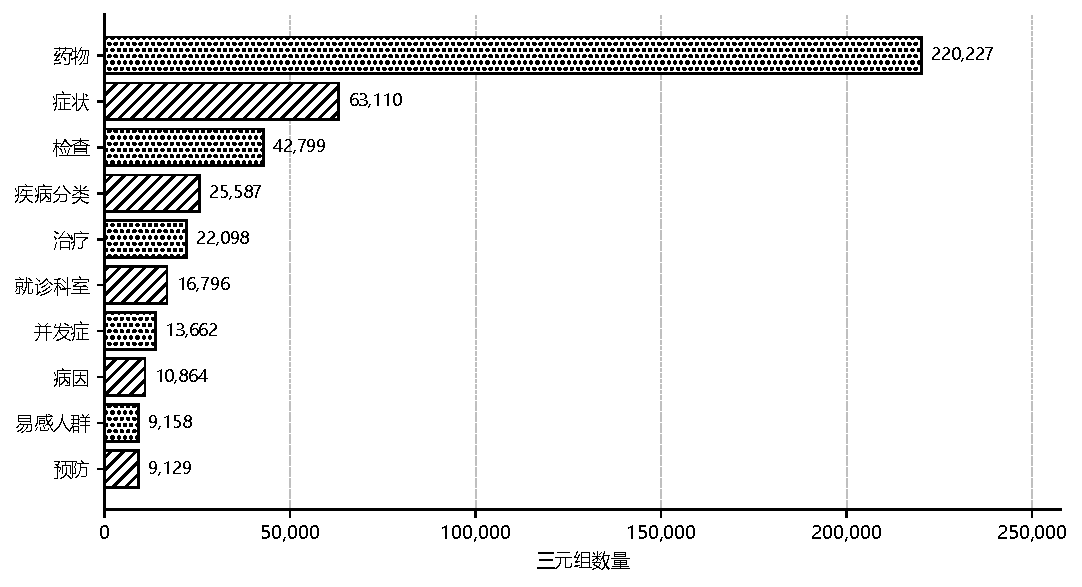
\includegraphics[width=0.88\textwidth]{figures/runtime_relation_distribution.pdf}
\caption{运行实例主要关系类型规模}
\label{fig:runtime-relations}
\end{figure}

运行数据中，药物关系约占全部三元组的一半，
症状、检查、疾病分类和治疗关系的数量居后但仍构成主要关系类别。
DataMate 增量事实作为独立来源进入同一统计口径，
这些来源继续沿用同一组查询工具和分析表。

\chapter{面向业务问题的受控分析}

\section{分析对象与访问入口}

任务三面向疾病事实和图谱统计，
支持疾病属性、实体关系、知识覆盖、来源构成和类别分布等问题。
正式查询链路由一个统一分析服务承接，
Nexent 任务三智能体和 Web 工作台是该服务的两个调用入口。
Nexent 适合用对话提出问题，工作台适合查看查询计划、结果数据、统计图和成果文件；
两者都经过同一语义规划、只读执行和结果组织流程。
图谱库用于关系子图和来源登记，分析库提供疾病事实表与统计查询；
统一分析服务把分析库返回的证据、图表和来源范围组织到同一分析结果中。

任务三的实现流程见图~\ref{fig:task3-pipeline}。
系统先把问题转换为一个或多个查询计划，
再执行安全检查和只读查询，
最后形成一条可复用的分析结果记录。

\begin{figure}[H]
\centering
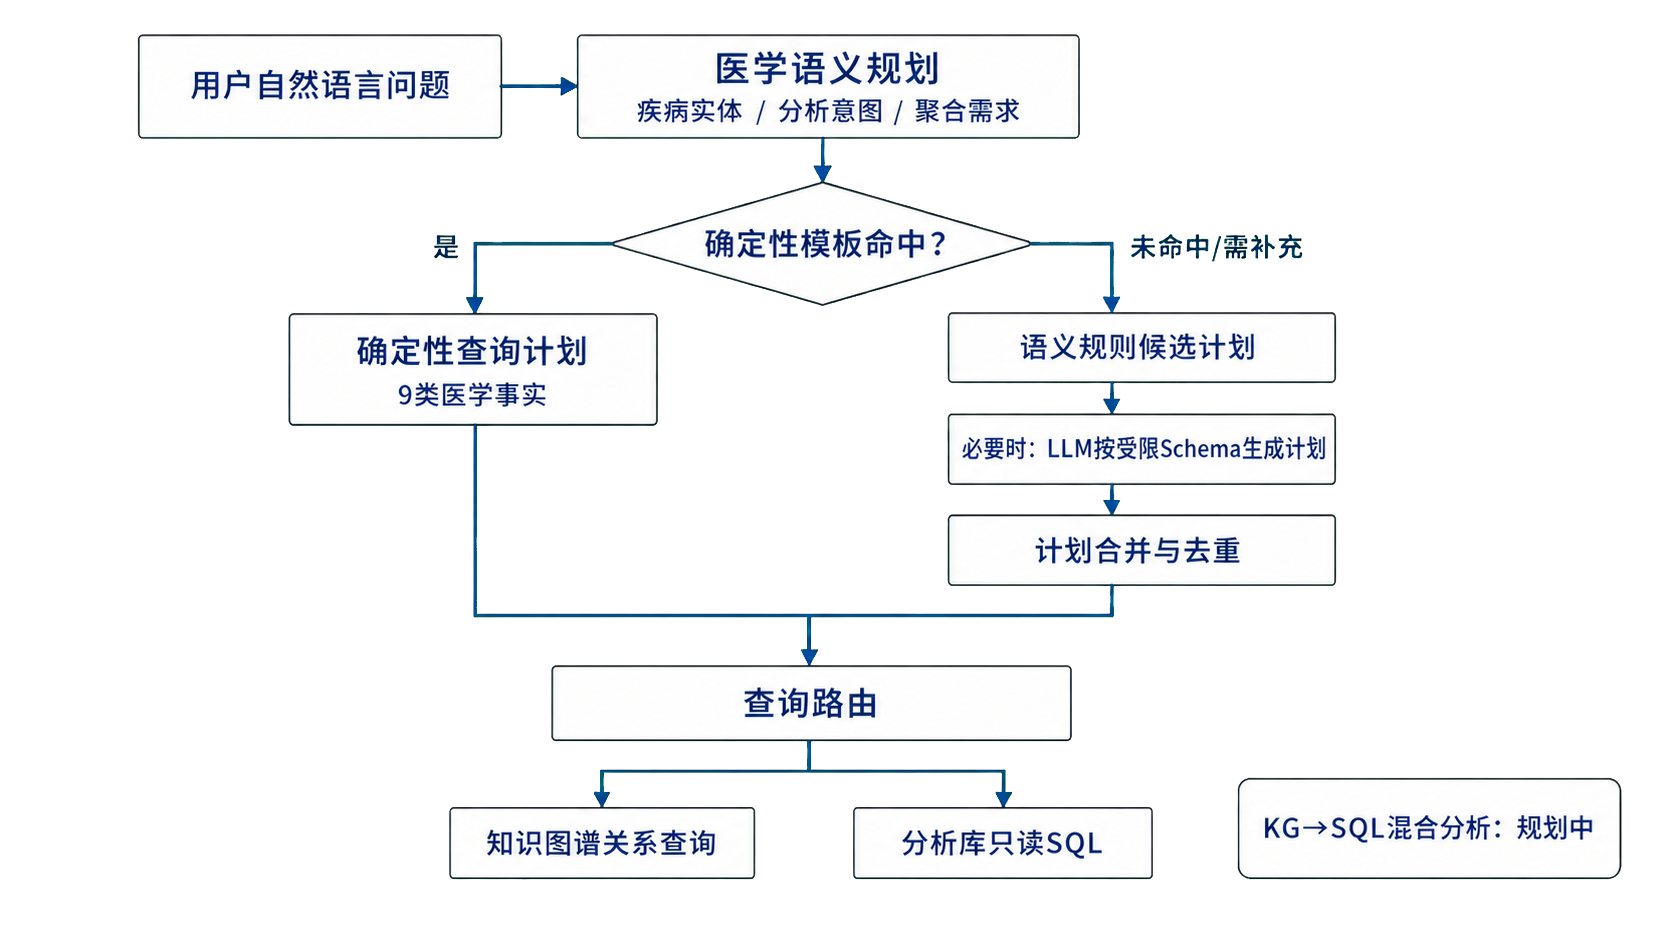
\includegraphics[width=0.90\textwidth]{figures/task3-planning.png}
\caption{任务三的语义规划与查询路由}
\label{fig:task3-pipeline}
\end{figure}

图~\ref{fig:task3-pipeline}把任务三的规划阶段拆成两条受控分支：
命中确定性模板时生成九类医疗事实查询计划，
未命中模板时先由语义层生成候选计划；
只有在语义层判定仍需补充且模型服务可用时，
才请求模型按 Schema 约束生成候选计划，
然后按 SQL 和数据源去重并限制查询数量。
任务三智能体在工具路由阶段再按问题类型选择知识图谱关系查询或统一只读 SQL 分析。
模型服务未配置或调用失败时，系统保留可验证的语义层结果并标记降级，
不会把模型未返回的内容当作查询结果。
图右下角的“KG$\rightarrow$SQL 混合分析：规划中”是后续扩展方向，
不属于当前实现，也不计入本报告的评测结果。

\section{基于语义规划的查询路由}

医疗语义层将自然语言中的疾病名称和关系意图映射到实际业务表。
系统从疾病主表中匹配名称，
当多个疾病名同时出现时优先采用更长、更具体的名称。
症状、药物、并发症、科室、检查、治疗、易感人群、病因和预防
分别对应 9 个事实定义，
每个定义明确目标表、疾病字段、结果字段、显示标题和默认排序。

“某病有哪些症状”“某病应该做哪些检查”等问题直接生成受控查询；
实体类型分布、关系类型分布和科室疾病分布使用预置统计视图。
对于包含多个条件或未命中模板的问题，
语义层先生成可验证的候选计划；
当问题仍需要开放式补充且模型服务可用时，
规划器才请求模型返回受限 JSON 查询计划，
并将模型计划与已识别的语义计划按 SQL 和数据源去重，
最终保留最多 4 项查询。
这套顺序使常用业务问题采用稳定模板，
复杂表达仍可扩展到受控查询；当模型服务不可用时，结果会明确标记为降级。

任务三智能体先判断用户要求的是疾病事实、图谱关系、数据来源还是统计分析，
再由任务级工具选择对应的只读能力。
疾病详情、统计、排名和解释类自然语言问题统一调用
\texttt{ask\_medical\_analytics}，进入同一个语义规划器和分析服务；
常见问题使用确定性模板，复杂问题再使用结构化查询计划。
关系子图和来源清单仍由专用工具直接读取对应的图谱表，
图谱关系查询与统计分析结果使用各自独立的结果口径。
因此，Nexent 的对话分析和工作台的可视化结果都遵循同一结果对象契约，
不会在两个入口各自维护一套自然语言查询执行逻辑。

代码上，\path{task3/runtime.py} 是服务装配入口。
Web 工作台通过 \path{analysis_runtime.py} 调用它，
MCP 通过 \path{mcp_server/tools/task3_runtime.py} 调用它。
\path{execute_nl2sql} 保留为兼容旧智能体配置的工具名，
但与 \path{ask_medical_analytics} 使用同一个服务实例、同一分析库和同一结果契约。
\path{query_disease_analytics} 只保留旧调用方所需的结构化字段投影，
不再作为任务三智能体的自然语言主路由。

智能体不会直接修改分析库。
涉及数据接入、重新建图或刷新来源的请求，
先进入任务二建图工具；
涉及查询的请求只能生成单条\texttt{SELECT}或\texttt{WITH}语句，
并由服务端执行表名、只读连接、时限和返回行数检查。
查询失败、数据不足或问题超出当前表结构时，
分析结果记录保存相应状态和口径说明，
回答只引用实际返回的数据。

\section{自然语言查询的只读执行}

查询安全模块要求 SQL 以 \texttt{SELECT} 或 \texttt{WITH} 开头，
并且只能包含一条语句。
注释、数据库附加、结构修改和数据写入关键字在执行前被拦截，
表名必须位于 17 个允许查询对象（14 张表和 3 个视图）的清单中。
SQLite 通过 URI 只读模式打开，
连接后再设置 \texttt{PRAGMA query\_only=ON}。

执行器为每项查询安装 5 秒进度中止条件，
最多返回 200 行；
一次分析最多执行 4 项查询。
每项结果保存标题、SQL、参数、列、数据行、返回数量和耗时，
单项查询的状态互相独立。
这些限制同时应用于语义模板和模型生成计划，
并由统一分析服务对两个调用入口执行。

\section{分析结果呈现}

分析服务根据查询标题与数据列组织文字回答，
原始返回行同步保留为结果表。
图表策略先读取用户是否明确要求图形，
再根据维度类型和记录数量选择展示形式。
时间字段才允许使用折线图；
类别比较使用条形图或柱状图；
构成比例使用环形图，并保留前 8 类、其余合并为“其他”。
条形图最多展示 20 类，柱状图最多 12 类，折线图最多 16 个点。

分析结果记录包含以下内容：

\begin{itemize}
  \item 用户问题、识别主题和查询计划；
  \item 每项查询的 SQL、参数、列和数据行；
  \item 文字回答、结果说明和数据口径；
  \item 图表类型、标题、维度字段、数值字段和截取规则；
  \item 分析标识、数据库文件名、查询数量、返回行数和执行耗时。
\end{itemize}

每次分析生成独立分析标识。
页面中的回答、结果表和统计图都读取同一对象，
导出模块也按该标识取得当前结果，
使屏幕展示与下载文件使用相同的数据行。
图~\ref{fig:task3-result-object} 展示从问题识别、查询计划到分析结果记录的具体映射。

\begin{figure}[H]
\centering
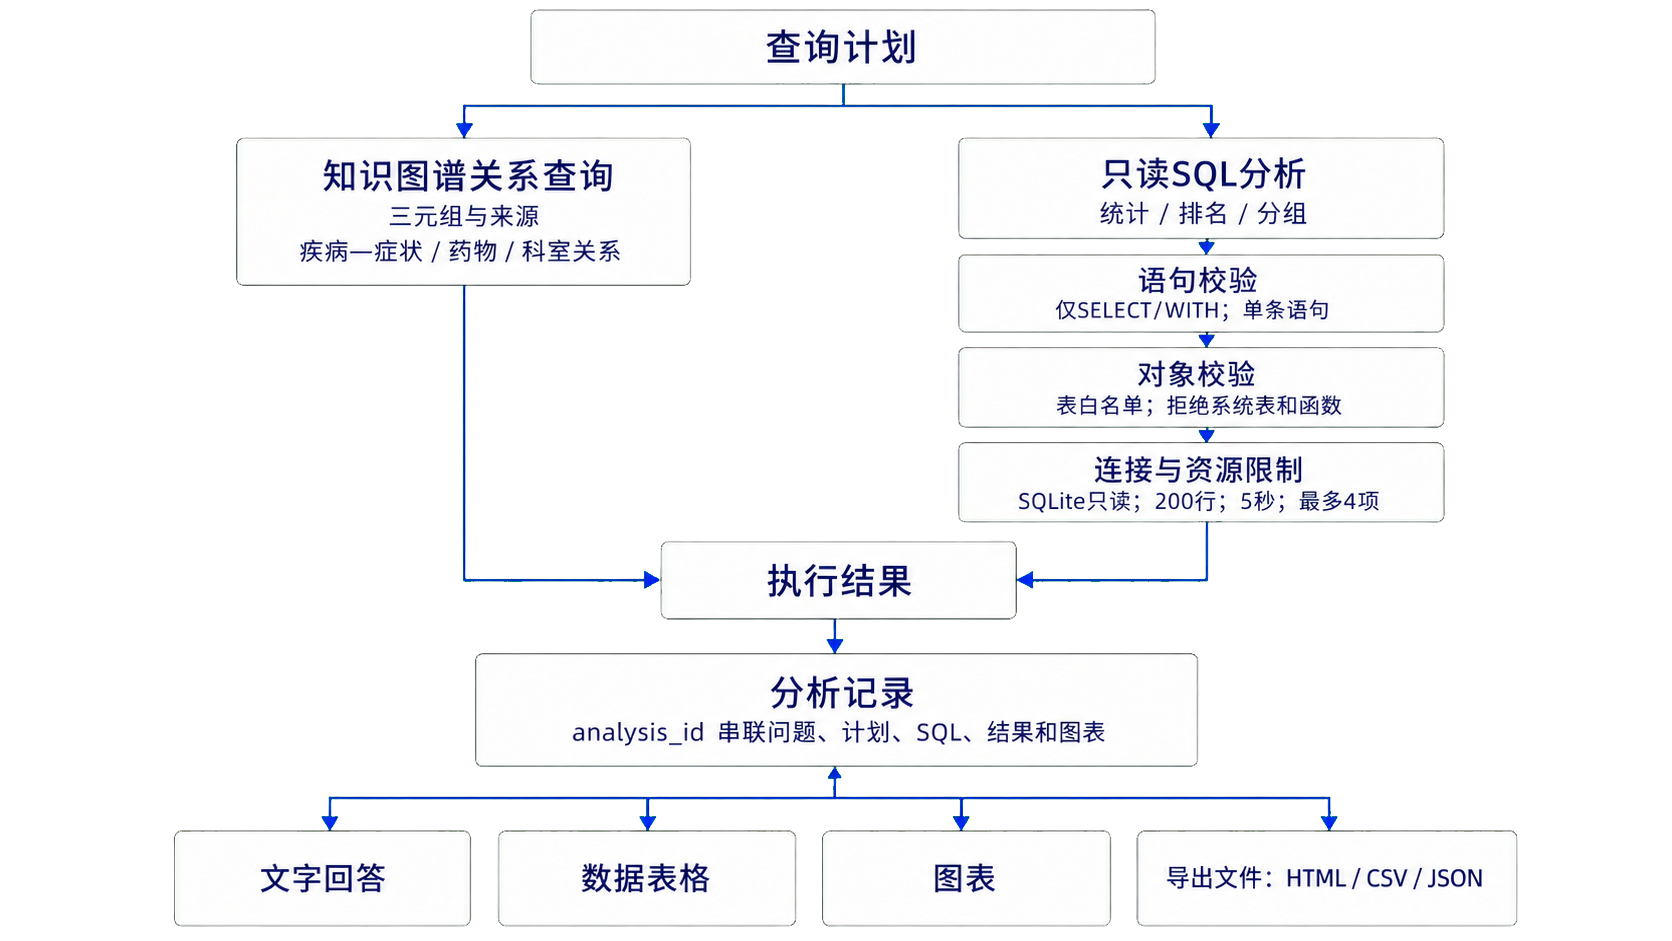
\includegraphics[width=0.90\textwidth]{figures/task3-execution-delivery.png}
\caption{任务三的受控执行与统一结果交付}
\label{fig:task3-result-object}
\end{figure}

图~\ref{fig:task3-result-object}说明两个查询分支如何汇入同一执行结果：
图谱关系查询工具面向疾病、症状、药物和科室关系，
统一分析服务面向疾病详情、统计、排名和分组问题；
SQL 分支依次通过语句、对象、连接和资源检查，
最后由同一分析记录驱动文字回答、数据表、图表和 HTML、CSV、JSON 导出。

图谱库与分析库承担不同职责，不能把两者的数量混写：
图谱库保存规范化实体、三元组和来源，
分析库保存由这些事实投影得到的疾病事实表和统计视图。
因此，图中的“图谱关系查询”不表示统计 SQL 直接读取三元组表；
统计、排名和分组问题仍在分析库上执行只读 SQL，
具体数量以同一运行核验快照中的数据表为准。

\section{知识图谱的关系浏览}

关系图直接读取图谱中的实体和三元组。
用户选择疾病后，
系统按症状、药物、检查、科室、治疗和并发症等关系展开相邻节点。
节点样式和图例在在线界面中区分实体类型，
节点数较多时按关系类型与数量限制展开。
导出的数据表以实体名称、关系名称、分组可靠性分和来源字段保存图中事实。
对任务二增量写入的关系，来源字段包含数据集、文件名、记录号和原文证据；
用户可以从图上的一条边回到任务一最终数据集中的具体文件与记录。

图谱浏览与统计分析可以在同一工作台切换。
关系图适合查看具体疾病的知识结构，
统计图适合比较实体类型、关系类型和来源贡献。
两种展示由同一工作台组织：关系图读取图谱库，统计图读取分析库；
用户能够从总体分布继续查看具体事实。

\section{分析成果导出}

报告模块从当前分析结果记录生成压缩包，
其中包含 HTML 报告、按查询拆分的 CSV 数据和“分析追溯”JSON。
HTML 保存问题、回答、查询步骤、结果表和图表说明；
每项查询单独生成 CSV；
JSON 保存分析计划、SQL、执行状态、来源和完整结果结构。
导出入口按分析标识读取页面已经展示的数据；
当标识对应的结果记录不可用时，服务返回状态信息，要求重新发起分析，
不会在导出阶段静默替换原结果。

HTML 适合离线阅读与成果交流，
CSV 可继续进入统计工具，
分析追溯 JSON 用于保存完整结果结构和接口联调。

\chapter{系统实现与部署}

\section{技术选型与运行依赖}

作品以 Python 实现智能体工具服务和医疗领域逻辑，
使用 FastMCP 暴露 MCP 接口，
使用两套 SQLite 数据库分别保存知识图谱和分析表。
DataMate 的数据集、文件、算子和任务状态由平台服务及 PostgreSQL 管理，
Nexent 负责智能体配置、模型调用和对话执行。
在线工作台采用轻量 HTTP 服务与 HTML、CSS、JavaScript，
关系图和统计图在浏览器中使用 SVG 绘制。

\begin{table}[H]
\centering
\caption{主要技术与用途}
\label{tab:technology-stack}
\begin{tabularx}{\textwidth}{L{3.2cm}L{4.0cm}Y}
\toprule
\textbf{技术或平台} & \textbf{对应架构层} & \textbf{项目用途} \\
\midrule
Nexent & 智能体层 &
配置三个专业智能体，绑定 MCP 工具并提供对话入口 \\
\addlinespace
DataMate & 服务层 &
管理数据集、文件、自定义算子和清洗任务 \\
\addlinespace
FastMCP & 接口层 &
注册任务一至任务三工具并返回结构化结果 \\
\addlinespace
Python & 服务层 &
实现格式处理、抽取校验、图谱事务、查询规划和成果导出 \\
\addlinespace
SQLite、PostgreSQL & 数据层 &
保存图谱事实、疾病分析表和 DataMate 平台数据 \\
\addlinespace
Docker Compose & 部署支撑 &
组织上游平台、MCP 服务、演示服务和数据卷 \\
\bottomrule
\end{tabularx}
\end{table}

\section{代码模块组织}

项目把协议入口、平台访问、业务编排、领域处理、数据存储和部署资产分开。
表~\ref{tab:module-map} 给出主要代码范围。
MCP 工具只负责参数接收、校验和结果返回，
跨步骤流程由任务服务编排，
平台调用进入客户端或适配模块，
实体、关系、分析计划等结构由领域模块统一表达。

\begin{table}[H]
\centering
\caption{主要代码范围与职责}
\label{tab:module-map}
\begin{tabularx}{\textwidth}{L{4.4cm}Y}
\toprule
\textbf{代码范围} & \textbf{职责} \\
\midrule
\repoPath{clients/} &
封装 Nexent 与 DataMate 的 HTTP 接口和身份配置 \\
\repoPath{mcp_server/tools/} &
注册智能体可调用的 MCP 工具，检查参数并整理返回结构 \\
\repoPath{mcp_server/task1/} &
数据集探查、混合格式编排、PDF 适配、状态和质量记录 \\
\repoPath{mcp_server/task2/}、\repoPath{mcp_server/kg/} &
医疗记录解析、知识抽取编排、图谱存储和分析表刷新 \\
\repoPath{core/} &
医疗抽取、九类实体校验、关系映射和图谱查询 \\
\repoPath{kg/} &
基础图谱导入、15 类关系映射和分析数据库构建 \\
\repoPath{operators/} &
DataMate 可注册的医疗数据处理与知识抽取算子 \\
\repoPath{task3/} &
统一分析服务、九类疾病事实语义层、查询计划、SQL 安全、图表策略和报告生成 \\
\repoPath{mcp_server/tools/task3_runtime.py}、\repoPath{demo/task3_interactive_demo/analysis_runtime.py} &
分别为 MCP 与 Web 入口装配同一分析服务，复用分析库路径、来源范围和大模型配置 \\
\repoPath{demo/} &
图谱浏览、数据分析和成果下载的在线工作台 \\
\repoPath{deploy/}、\repoPath{scripts/} &
环境检查、组件安装、平台注册、服务启动和验收 \\
\bottomrule
\end{tabularx}
\end{table}

\section{平台接入与智能体发布}

DataMate 接入分为数据集访问和算子运行两部分。
客户端通过平台接口解析数据集名称与标识、上传文件、读取文件清单，
并登记最终交付数据集；
任务服务创建算子实例与清洗任务，轮询任务状态并取得目标数据集。
文件内容通过 DataMate 的文件记录和数据卷读取，
数据集、任务和产物仍由平台统一管理。
医疗术语整理、表格列清理、JSON 字段清理和知识抽取算子
以算子代码和描述文件的形式注册到 DataMate，供任务调用。
任务一在线流程直接创建 DataMate 清洗任务；
任务二在线建图入口调用共享抽取服务，算子接口与该服务共用抽取模型和校验模块。

Nexent 接入分为 MCP 工具注册和智能体配置更新。
部署时先在 Nexent 建立三个智能体入口并配置所用模型。
发布脚本按智能体标识或名称读取当前版本，
从 MCP 工具清单中解析工具标识，
更新职责说明和工具绑定后发布新版本。
已有对话入口可以沿用原智能体标识，
工具集合和提示内容由脚本统一更新，数据集、任务和分析标识按工具返回值传递。
项目代码通过客户端和 MCP 接口连接两套上游平台，
医疗领域模块保持在独立目录中。

智能体配置包含职责提示、约束提示、工具集合和可选的少样本示例。
职责提示说明角色负责的业务范围，
约束提示规定工具调用顺序、真实标识传递、只读边界和错误反馈，
工具集合由 MCP 服务扫描结果绑定到已发布版本。
这些配置决定模型能够看到哪些工具，
但不替代服务端的参数校验和数据库安全检查。

项目中的三个概念具有不同职责。
FastMCP 是运行 MCP 服务并注册工具的服务框架；
MCP 工具是智能体可以调用的一个结构化工具入口；
DataMate 算子是平台内执行单个数据变换的处理单元。
例如，\path{run_task1_mixed_cleaning} 是 MCP 工具，
它在服务内部按格式创建 DataMate 清洗任务，
清洗任务再组合医疗术语规范、字段清理和文本质量处理等算子。

\section{系统部署架构}

运行环境包括 Nexent、DataMate 等上游服务，
以及 MediFlow MCP 服务、可视化服务和数据存储，
见图~\ref{fig:deployment}。
MCP 服务和可视化服务通过环境配置访问上游平台与数据库，
数据文件保存在独立卷或项目数据目录。

\begin{figure}[H]
\centering
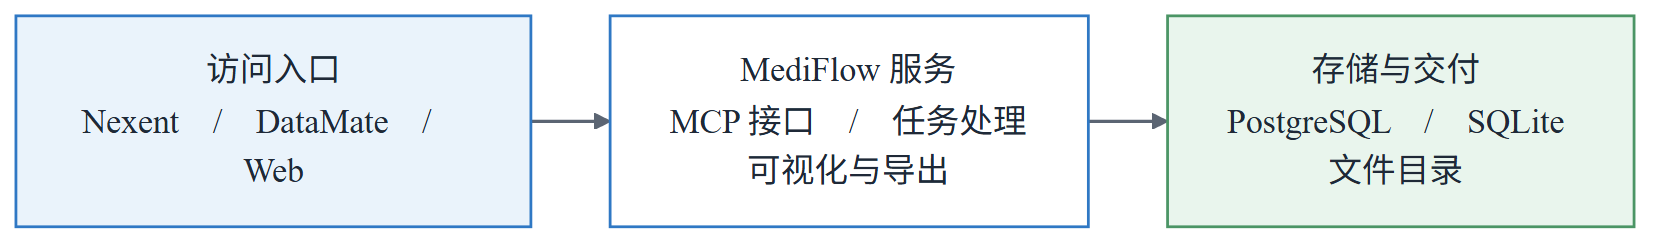
\includegraphics[width=0.90\textwidth]{figures/mermaid_deployment.png}
\caption{MediFlow 运行部署关系}
\label{fig:deployment}
\end{figure}

公开入口包括
\href{https://demo.mashiro.xin/}{MediFlow 工作台}、
\href{https://nexent.mashiro.xin/}{Nexent} 和
\href{https://datamate.mashiro.xin/}{DataMate}。
工作台用于查看图谱、提交分析问题并导出成果，任务三查询进入与 Nexent 相同的统一分析服务；
Nexent 提供三个专业智能体；
DataMate 用于管理数据集、算子和处理任务。

\section{项目交付资产}

当前运行实例建立在已准备好的 Nexent 与 DataMate 环境上。
仓库中的 \repoPath{deploy/} 目录按顺序保存环境检查、Python 依赖、
DataMate 算子注册、知识图谱与分析库构建、
MCP 服务启动与工具扫描、Nexent 智能体发布、
工作台启动和服务检查脚本。

部署目录同时提供分步脚本和顺序入口，
可以按组件安装，也可以按完整流程执行。
配置示例集中列出平台地址、数据库路径、模型接口和功能开关，
服务连接参数由部署环境注入。
图谱库与分析库由构建脚本生成，
MCP 服务和工作台在启动时读取同一组数据库配置。

\section{异常记录与故障定位}

\enlargethispage{2\baselineskip}
任务一把错误定位到文件下载、DataMate 子任务、PDF 解析或结果登记，
并保留已完成格式分组的结果；
任务二按记录返回解析与抽取状态，
图谱写入采用事务，分析刷新只在新增事实提交后执行；
任务三把计划、校验、查询和导出状态分别写入分析结果记录，
各单项查询结果独立保存。
对话入口和工作台读取同一结构化状态，
用户可以定位到数据集、文件、记录或查询。

\chapter{测试与性能分析}
\label{chap:testing}

\section{测试范围与数据集}

测试围绕三个功能阶段展开：
任务一检查五类文件路由、PDF 解析适配和原有格式兼容性；
任务二检查记录解析、级联抽取、可靠性分级和图谱入库；
任务三使用八个在线业务场景验证语义规划、只读查询、结果组织和统计图生成，
并通过 MCP 传输层核对统一分析入口和兼容入口的结果契约。
任务二当前提供 32 项独立自动化回归用例；任务一、任务三按各自评测脚本另行执行；
业务查询通过公开工作台接口连续请求三次并记录返回行数与响应时间。

\section{智能体工具调用核验}

智能体行为核验关注三个可观察结果：
工具选择是否与用户目标一致，
调用是否使用了真实的数据或查询参数，
返回结果是否包含回答所需的结构化事实。
分别执行统一医学分析查询和数据来源查询，
前者选择 \path{ask_medical_analytics}，
后者选择 \path{get_medical_data_sources}。
两次调用均返回对应的结构化数据，
最终回答仅采用工具返回的数量和医学事实。

\begin{table}[H]
\centering
\caption{代表性智能体工具路由核验}
\label{tab:agent-route-check}
\begin{tabularx}{\textwidth}{L{3.3cm}L{4.0cm}Y}
\toprule
\textbf{用户目标} & \textbf{实际选择的工具} & \textbf{可核对结果} \\
\midrule
查询肺不张症状 & \path{ask_medical_analytics} &
返回确定性查询计划、20 行证据、SQL 和分析追溯信息 \\
查询当前登记来源 & \path{get_medical_data_sources} &
返回来源总数、来源列表和记录规模 \\
\bottomrule
\end{tabularx}
\end{table}

工具路由与后端处理保持分层：
智能体只选择任务级入口，
工具服务负责参数校验和状态整理；
任务三的查询、图表和导出统一进入分析服务，
后续的算子执行、图谱事务或只读查询由确定性服务完成。
因此，路由核验与任务一、任务二和任务三的功能测试分别检查不同层次。

运行态还通过 MCP 的 Streamable HTTP 接口列出 19 个工具，
分别调用 \path{ask\_medical\_analytics} 和兼容的
\path{execute\_nl2sql}。
同一问题两次均返回成功、确定性 NL2SQL 规划和 20 行结果，
两次生成的 SQL 相同，并同时包含来源范围和执行追溯字段。
工作台 \path{/api/query} 也返回相同的分析状态和 20 行证据。
Nexent Agent 对话已实际选择 \path{ask\_medical\_analytics}，
但当前事件流只返回最终文本，没有返回可验证的结构化分析对象；
网关因此使用同一分析服务回退并标记降级。
这证明了服务链路统一，不把该次 Agent 对话描述为结构化事件闭环通过。

\section{任务一输入路由测试}

\repoPath{tests/task1/test_pdf_support.py} 包含 9 项自动化用例，
覆盖 PDF 接入新增逻辑及 TXT、CSV、JSON、JSONL 原有路由。
测试使用模拟的 MinerU 响应，
检查本地接口转换、格式路由与产物转换逻辑。
全部用例执行通过，分组结果见表~\ref{tab:unit-test-results}。

\begin{table}[H]
\centering
\caption{任务一格式与 PDF 路由测试结果}
\label{tab:unit-test-results}
\begin{tabularx}{\textwidth}{L{3.1cm}Y C{2.0cm}}
\toprule
\textbf{测试分组} & \textbf{覆盖内容} & \textbf{结果} \\
\midrule
格式路由与兼容性 &
PDF 分类、二进制预览保护、原有四类格式分组、
结构化处理链保持、PDF 转文本后复用文本链 &
5/5 通过 \\
\addlinespace
MinerU 接口适配 &
签名上传与任务轮询、结果下载、Markdown 正文转换、
TXT 产物与解析信息生成 &
3/3 通过 \\
\addlinespace
PDF 服务可用性路由 &
远程解析可用性识别与处理链选择 &
1/1 通过 \\
\midrule
合计 & 9 项测试 & 9/9 通过 \\
\bottomrule
\end{tabularx}
\end{table}

这组用例覆盖的结果为：
新增 PDF 分支保持了四类原有格式的分组和结构化处理链，
解析产物能够转为 TXT 并继续进入既有文本清洗流程，
上传、轮询和下载状态也能够转换为任务一统一结果。

\section{任务二抽取回归测试}

任务二的 32 项用例覆盖级联抽取和工具层的异常保护。
其中 8 项检查模型服务降级、空结果和未知可靠性等级的安全返回，
18 项检查长实体匹配、分段疾病归属、统一实体门禁和缺口候选，
6 项检查离线优先、批处理范围、复核决定和未复核候选的入库状态。
测试使用固定文本和模拟模型返回，
不依赖外部模型服务；本组 32 项用例在同一代码仓环境中全部通过。

\begin{table}[H]
\centering
\small
\caption{任务二自动化测试结果}
\label{tab:task2-test-results}
\begin{tabularx}{\textwidth}{L{3.0cm}Y C{2.0cm}}
\toprule
\textbf{测试分组} & \textbf{覆盖内容} & \textbf{结果} \\
\midrule
工具防护与降级 &
模型服务异常、空结果、未知可靠性等级和混合方式降级 & 8/8 通过 \\
\addlinespace
级联语义回归 &
长实体优先、分段疾病归属、统一实体门禁与原文范围保持 & 18/18 通过 \\
\addlinespace
级联流程与入库 &
离线优先、复核队列、批处理边界和未复核候选处理 & 6/6 通过 \\
\midrule
合计 & 32 项测试 & 32/32 通过 \\
\bottomrule
\end{tabularx}
\end{table}

\section{任务二固定留出集评测}

功能回归用于检查处理链是否按预期运行，质量评测则采用固定留出集计算实体和关系抽取指标。
本次评测使用 CMeEE 的 2\,500 条实体样本和 CMeIE 的 1\,793 条关系样本，
采用严格匹配统计精确率、召回率和 F1，并同步记录单条记录的中位耗时与 P95 耗时。
评测后端为 \texttt{offline}，结果对应词典、规则和版本配置均已固定。

\begin{table}[H]
\centering
\small
\caption{任务二固定留出集离线评测结果}
\label{tab:task2-holdout}
\begin{tabularx}{\textwidth}{L{2.1cm}L{2.3cm}C{1.1cm}C{1.2cm}C{1.2cm}C{1.2cm}Y}
\toprule
\textbf{评测对象} & \textbf{数据集} & \textbf{样本数} & \textbf{精确率} & \textbf{召回率} & \textbf{F1} & \textbf{耗时/ms（P50/P95）} \\
\midrule
实体识别 & CMeEE 固定留出集 & 2\,500 & 53.94\% & 28.97\% & 37.70\% & 2.26 / 33.84 \\
关系抽取 & CMeIE 固定留出集 & 1\,793 & 74.34\% & 7.92\% & 14.31\% & 7.84 / 48.21 \\
\bottomrule
\end{tabularx}
\end{table}

实体识别结果反映词典匹配对高频术语的覆盖，关系抽取结果反映当前离线规则在严格关系匹配下的有效输出。
两项指标共同作为任务二离线基线，后续模型增强评测沿用相同样本划分和匹配规则，保证结果可比较。

固定留出集用于正式报告；开发过程中另取 CMeEE、CMeIE 各 100 条做同批工程回归，
用于快速判断级联修改是否同时改善离线与混合链。该小样本不替代固定留出集成绩。
统一低可靠实体与模型补漏实体的门禁后，实体识别的混合方式达到
63.93\% 精确率、58.42\% 召回率和 61.05\% F1，
均高于同批离线方式的 60.80\%、39.19\% 和 47.66\%。
关系抽取增加分段疾病标题继承后，离线方式为
78.43\%/12.99\%/22.28\%，混合方式为
79.31\%/14.94\%/25.14\%；模型补充的关系保持严格证据门禁，
本轮 100 条记录未出现模型调用错误，也未写入知识图谱或刷新分析库。

\section{知识库与分析库核验}

公开工作台的数据概览返回 14\,408 个疾病条目、79\,605 个实体、
445\,820 条三元组、445\,210 条疾病事实、3\,836 条质量记录和 6 个来源。
基础结构化知识、CMeIE 关系与 DataMate 增量事实之和为 445\,820，
与图谱三元组总数一致。
分析数据库按疾病事实口径生成 445\,210 条记录。

\begin{table}[H]
\centering
\caption{知识库与分析库检查结果}
\label{tab:runtime-check}
\begin{tabularx}{0.86\textwidth}{Y C{3.0cm} C{2.2cm}}
\toprule
\textbf{检查项目} & \textbf{数量或状态} & \textbf{结果} \\
\midrule
图谱实体 & 79\,605 & 可查询 \\
图谱三元组 & 445\,820 & 可查询 \\
来源分项合计 & 445\,820 & 与总数一致 \\
疾病事实 & 445\,210 & 可查询 \\
分析成果导出 & HTML、CSV、JSON & 可用 \\
\bottomrule
\end{tabularx}
\end{table}

\section{在线查询验证}

业务查询覆盖疾病的症状、检查、治疗、科室和药物五类属性，
以及科室分布、实体类型分布和关系类型分布三类统计问题。
每个问题在同一公开工作台接口上连续请求三次，
表~\ref{tab:online-query-results} 给出页面实际展示行数、
三次请求的中位响应时间和波动范围。
响应时间包含 HTTPS 传输、语义规划、SQLite 查询和结果组织；
表中“范围”为三次请求的最小值至最大值，
本表用于描述该服务实例的响应情况，解释范围限定为当前运行配置。

\begin{table}[H]
\centering
\small
\caption{在线业务查询与响应时间}
\label{tab:online-query-results}
\begin{tabularx}{\textwidth}{L{3.0cm}Y C{1.5cm} C{1.8cm} C{2.1cm}}
\toprule
\textbf{场景} & \textbf{测试问题} & \textbf{行数} &
\textbf{中位/ms} & \textbf{范围/ms} \\
\midrule
疾病症状 & 肺炎有哪些症状？ & 40 & 719 & 637--1\,028 \\
疾病检查 & 肺炎应该做哪些检查？ & 40 & 576 & 546--689 \\
疾病治疗 & 肺炎有哪些治疗方法？ & 34 & 583 & 530--631 \\
就诊科室 & 肺炎应该挂哪个科室？ & 12 & 609 & 568--610 \\
常用药物 & 肺炎常用哪些药物？ & 40 & 824 & 747--852 \\
科室分布 & 疾病在各科室的分布情况如何？ & 30 & 570 & 537--588 \\
实体分布 & 医疗知识图谱中各类实体数量是多少？ & 12 & 553 & 540--580 \\
关系分布 & 知识图谱中不同关系类型的数量是多少？ & 16 & 539 & 535--558 \\
\bottomrule
\end{tabularx}
\end{table}

八个问题均由医疗语义层完成规划并返回结构化结果。
五类疾病属性查询生成文字回答和结构化结果表，
三类分布查询同时生成统计图。
连续请求的中位时间位于 539--824\,ms，
药物与症状查询各返回 40 行；
关系分布查询的观测中位数最低；表中数据用于描述总体响应，不拆分网络、规划和查询各阶段的耗时。

\section{任务三 NL2SQL 执行评测}

在线业务核验关注服务是否能完成一次端到端请求，
NL2SQL 评测则单独检查自然语言问题能否生成可执行查询并返回正确结果。
评测目录包含 133 道题：开发集 40 题，测试集 93 题；
题目覆盖单表筛选、聚合统计、分组统计、Top-K 排序、多条件查询、多表联查和复杂综合七类 SQL 结构。
构建脚本先在真实的 \texttt{task3\_analytics.db} 上执行 Gold SQL，
再保存自然语言问题和 Gold Result，
因此每道题都有可复核的查询结果和数据口径。

评测主指标为执行结果准确率：
系统生成的 SQL 在同一分析库执行后，
返回行按多重集合比较，行内重复记录保留，顺序差异不影响判定。
该指标回答的是“查询结果是否正确”，
不等价于 SQL 字符串相同，也不衡量知识库检索、来源引用、图表样式或 Nexent 完整对话质量。
复现入口为 \texttt{evaluation/task3/run\_benchmark.py}，
题目、数据库和评测输出分别保存在 \texttt{evaluation/task3/} 下。

\begin{table}[H]
\centering
\small
\caption{任务三 NL2SQL 执行准确率与评测口径}
\label{tab:task3-nl2sql-summary}
\begin{tabularx}{\textwidth}{L{3.0cm}C{1.7cm}C{1.7cm}Y}
\toprule
\textbf{运行对象} & \textbf{正确/总题数} & \textbf{执行准确率} & \textbf{口径说明} \\
\midrule
开发集初始方案 & 25/40 & 62.5\% & 开发集初始运行，用于识别模板覆盖和查询规划缺口 \\
开发集方案验证 & 38/40 & 95.0\% & 在开发集上验证语义模板与结构化计划的改动 \\
测试集设计基线 & 57/93 & 61.3\% & 测试集首次运行，未根据测试失败题型调整 \\
测试集回归复核 & 89/93 & 95.7\% & 已使用测试失败题型信息，属于回归复核，不是独立盲测 \\
\bottomrule
\end{tabularx}
\end{table}

表~\ref{tab:task3-nl2sql-summary} 说明，测试集设计基线低于赛题要求的 85\%，
回归复核达到 95.7\%。
回归复核中，聚合统计、分组统计、多条件查询、Top-K 排序和多表联查均达到 100\%；
复杂综合由 27.3\% 提升到 63.6\%，仍有 4 道题未通过。
这组结果支持“统一语义模板和受控查询计划能覆盖固定分析问题”的工程判断，
但不能把回归复核结果解释为对未见问题的泛化准确率。

\begin{table}[H]
\centering
\small
\caption{测试集按题型的 NL2SQL 执行准确率}
\label{tab:task3-nl2sql-by-type}
\begin{tabularx}{\textwidth}{L{2.8cm}C{1.1cm}C{1.8cm}C{1.8cm}Y}
\toprule
\textbf{题型} & \textbf{题数} & \textbf{设计基线} & \textbf{回归复核} & \textbf{结果解释} \\
\midrule
单表筛选 & 17 & 100.0\% & 100.0\% & 基本疾病属性查询覆盖稳定 \\
聚合统计 & 17 & 58.8\% & 100.0\% & 聚合字段和排序口径经模板固化 \\
分组统计 & 14 & 64.3\% & 100.0\% & 分组、排序和限制条件覆盖完整 \\
多条件查询 & 13 & 53.8\% & 100.0\% & 多条件过滤和子查询错误得到修正 \\
Top-K 排序 & 12 & 83.3\% & 100.0\% & 排序方向和限制条数得到统一 \\
多表联查 & 9 & 11.1\% & 100.0\% & 联接键和连接路径是初始方案的主要缺口 \\
复杂综合 & 11 & 27.3\% & 63.6\% & 多跳关联、比例和综合聚合仍是当前弱项 \\
\midrule
合计 & 93 & 61.3\% & 95.7\% & 回归复核结果含测试集失败信息 \\
\bottomrule
\end{tabularx}
\end{table}

\textbf{评测结论。}
任务三目前可以稳定处理评测集中的常见疾病属性和固定统计结构，
复杂综合问题仍需要人工检查查询计划和结果口径。
该评测证明的是分析库上的 SQL 执行一致性，
任务三完整链路还需要结合 Nexent 工具调用、来源解释和工作台展示进行独立验收。

\section{阶段耗时与性能控制}

三个阶段具有不同的性能特征。
任务一的时间主要由文件下载、DataMate 算子任务和 PDF 解析组成，
系统按格式独立组织子任务，文件数超过 50 时转入后台；
任务二按记录完成抽取与校验，
写入采用数据库事务，并且只在产生新三元组时刷新分析库；
任务三由统一分析服务读取本地分析数据库，
通过模板或结构化计划、只读连接、5 秒中止条件和 200 行上限控制单次负载。

\begin{table}[H]
\centering
\caption{三阶段耗时记录与控制方式}
\label{tab:performance-controls}
\begin{tabularx}{\textwidth}{L{2.3cm}L{5.3cm}Y}
\toprule
\textbf{阶段} & \textbf{主要耗时} & \textbf{控制方式} \\
\midrule
数据处理 &
文件传输、DataMate 算子、PDF 版面解析、结果汇聚 &
按格式拆分任务；大数据集后台执行；保存分组进度 \\
\addlinespace
知识构建 &
逐记录抽取、实体关系校验、图谱写入、分析表刷新 &
轮转取样；事务写入；有新增事实时刷新分析库 \\
\addlinespace
分析查询 &
语义规划、SQLite 查询、回答与图表数据组织 &
模板优先；最多 4 项查询；5 秒中止；最多 200 行 \\
\bottomrule
\end{tabularx}
\end{table}

当前八类在线查询的中位响应时间为 539--824\,ms，
本次观测的最大值为 1\,028\,ms；
该结果用于描述当前服务实例的响应情况。
任务一与任务二涉及外部平台、文档解析和知识抽取，
系统返回结构已分别记录分组耗时、逐记录耗时、入库数量和刷新耗时，
这些字段为任务一和任务二在相同数据规模、配置和部署条件下的后续比较提供统一口径。

\chapter{关键设计与实现特点}

前面章节已经说明 MediFlow 的背景、整体设计、三项任务、实现和测试结果。
本章从系统设计角度提炼五个贯穿三项任务的技术决策，
说明它们分别解决了什么问题、在本项目中如何落地、
以及给整个系统带来了哪些具体收益。

\section{MCP 工具与平台边界}

赛题要求基于 Nexent 构建智能体，基于 DataMate 完成数据处理。
项目实现将平台访问、领域规则和智能体配置拆成三层：
Nexent 只负责理解用户任务和选择工具，
不接触 DataMate 的接口细节；
MCP 工具服务负责参数校验和结果整理，
内部再调用 DataMate 客户端和领域处理模块。
三个已发布智能体和自定义智能体均通过 MCP 工具名称绑定相应功能，
工具的参数约定和服务端校验保持一致。

\begin{table}[H]
\centering
\caption{三层职责划分}
\label{tab:three-layer}
\begin{tabularx}{\textwidth}{L{2.8cm}L{4.0cm}Y}
\toprule
\textbf{层次} & \textbf{运行载体} & \textbf{负责的内容} \\
\midrule
任务理解与对话 & Nexent 智能体 & 判断用户意图、选择工具、组织回复 \\
\addlinespace
协议与编排 & MCP 工具服务 & 参数检查、流程编排、结果汇总 \\
\addlinespace
平台执行与领域规则 &
DataMate + MediFlow 服务 &
数据集操作、清洗任务、知识抽取、SQL 安全 \\
\bottomrule
\end{tabularx}
\end{table}

因此，DataMate 接口变化由客户端适配层承接，
领域规则变化由服务模块承接，
智能体配置只保存角色提示、约束提示和工具绑定。
新增智能体时绑定已有 MCP 工具即可，
无需在提示词中重复写入 DataMate 调用细节。

\section{阶段标识与结果追踪}

数据处理、知识构建和分析查询三个阶段，
上下游之间需要传递数据集、文件、三元组和查询表等信息。
项目让每个阶段产生持久化标识，
下一个阶段凭标识读取上一个阶段的结构化结果：

\begin{itemize}
  \item 任务一向 DataMate 登记交付数据集，返回数据集标识；
  \item 任务二接收数据集标识，读取实际文件，
        入库时为每条三元组记录来源标识和文件标识；
  \item 任务三每次分析生成分析标识，
        将问题、SQL、数据行和图表说明打包为结构化对象。
\end{itemize}

这套标识串联形成三个具体结果：
第一，任务二不需要知道任务一用了哪些算子，
只需要一个数据集标识就能读取清洗结果；
第二，任务三的图表和导出文件均按同一个分析标识读取结果记录中的数据行；
第三，三元组的来源标识可用于查询原始文件，
分析标识可用于核对对应的查询计划和 SQL。

\section{离线优先的级联抽取}

医疗实体和关系抽取是任务二的核心环节。
将模型调用作为唯一抽取路径会带来两个实际限制：
一是模型服务波动或超时时整个抽取管道会中断；
二是批量处理会增加模型调用次数和等待时间，
在公开知识资源批量导入时成本很高。

MediFlow 为抽取服务提供三种执行方式：
本地词典与规则、大模型、以及离线优先的级联方式。
离线方式加载独立维护的约 3.17 万条医学术语词典和关系规则，
不调用外部模型，识别结果在相同输入和词典版本下可复现；
模型方式处理需要语义判断的文本；
级联方式先完成离线全量扫描，再按候选可靠性和句子覆盖情况决定模型复核或补充的范围。
三种方式通过同一组实体、关系和三元组字段提供结果，
上层编排逻辑不需要区分当前使用的是哪种方式。

在批量导入公开知识时可以显式使用离线方式，减少外部模型依赖；
任务二在线入口默认使用级联方式，
高可靠事实直接进入统一校验，中可靠候选进入复核，低可靠候选不进入主图谱；
对离线链路未覆盖但含有医疗提示词的句子，模型只返回原文直接支持的补充事实。
模型服务不可用时，系统保留已完成的离线结果并返回错误状态，
接口超时只影响对应的模型补充步骤。

在固定划分的离线评测中，CBLUE 的 CMeEE 实体识别评测集包含 2\,500 条样本，
实体识别精确率为 56.50\%、召回率为 29.57\%、F1 为 38.82\%；
CMeIE 评测集包含 1\,793 条样本，
关系抽取精确率为 11.46\%、召回率为 17.93\%、F1 为 13.98\%。
该结果用于说明当前离线链路的覆盖范围，
级联设计则把模型调用限制在缺口句和需复核候选上，
同时保留离线结果的可复现性、来源字段和原文片段。

\section{结构保持的数据处理}

项目输入同时包含 CSV 表格、JSON 对象和 JSONL 记录。
系统没有把所有输入先合并为无结构文本，
而是按格式保留列名、键名、嵌套层次和记录边界，
使后续知识抽取仍可按字段读取内容。

结构保持规则如下：
CSV 清洗时保留表头和行列位置，
JSON 清洗时保留键名和嵌套层次，
JSONL 清洗时保留逐行记录边界。
清洗完成后，汇聚步骤会对各格式产物重新解析检查：
CSV 重新读取表头确认列数一致，
JSON 和 JSONL 重新解析确认结构合法，
通过后才登记到最终数据集。
PDF 解析为文本后也保留源文件名，
知识抽取时可以区分哪些事实来自研文献、哪些来自表格数据。

由此，任务二在读取清洗结果时，
可以按字段取特定列的内容，
可以知道这条记录来自 CSV 的哪一行哪个文件。
这些信息会随来源字段和原文片段进入知识抽取结果。

\section{只读查询安全}

任务三需要根据自然语言问题执行 SQL 查询。
NL2SQL 的研究重点通常放在生成 SQL 的准确率上，
在一个需要公开展示的系统中，
SQL 的执行安全同样关键。
错误的 DELETE、多语句拼接、或者对系统表的访问，
都可能造成数据损坏或信息泄露。

MediFlow 将安全限制落实在三个层面：

\begin{itemize}
  \item \textbf{语句层}：只接受单条 SELECT 或 WITH 语句，
        拒绝多语句、注释注入和结构修改关键字；
  \item \textbf{对象层}：表名必须落在 17 张业务表和统计视图的允许清单中，
        跨库附加、系统表访问和自定义函数调用在解析阶段拦截；
  \item \textbf{连接层}：SQLite 以 URI 只读模式打开，
        连接后立即设置 \texttt{PRAGMA query\_only=ON}，
        即使前两层被绕过，数据库引擎本身也会拒绝写操作。
\end{itemize}

此外，每次分析最多执行 4 项查询、每项最多返回 200 行、
每项查询安装 5 秒进度中止条件。
这些限制的直接目的在于限制单次请求的资源占用，
避免异常查询长时间占用数据库连接。

这套三层安全方案同时服务于 Nexent 查询工具和独立工作台，
两个入口使用同一组执行规则。
八类业务查询的连续三轮测试（第七章）表明，
响应时间和返回行数见表~\ref{tab:online-query-results}。

\chapter{开源协作与工程交付}

\section{团队协作分工}

项目采用核心开发者主导、团队成员按专题协作的方式。
核心开发者承担总体架构、主要功能实现、DataMate 与 Nexent 接入、
数据库构建、工作台和部署；
团队成员参与赛题需求整理、上游项目阅读、数据来源整理、
测试问题设计、页面体验和提交材料编写。
功能范围由团队共同讨论，
代码实现由核心开发者集中维护，
使三项任务在数据结构和接口风格上保持一致。

代码仓按功能分支组织改动，
每项功能同步整理源码、配置示例、测试、部署脚本和说明文档。
平台接口与真实业务场景先在运行环境完成验证，
再形成可重复部署的项目资产。

\section{上游调研与方案形成}

团队先按赛题三项任务阅读 Nexent 与 DataMate 的官方文档和源代码。
对 Nexent 的调研集中在智能体版本、工具扫描、MCP 绑定和对话执行；
对 DataMate 的调研集中在数据集、文件记录、算子实例、清洗任务和目标数据集。
结合平台接口后确定：
DataMate 承载文件与算子处理，
Nexent 承载三个专业智能体，
项目 MCP 服务提供医疗领域功能。

随后围绕医疗数据的实际结构确定数据方案。
公开疾病知识与 CMeIE 关系用于构建基础图谱，
DataMate 结果作为独立来源增量写入；
图谱库保存规范化事实，
分析库保存面向疾病查询的派生表；
Python 与 FastMCP 实现服务，
SQLite 满足当前知识规模下的部署和只读分析，
独立工作台集中展示图谱、统计结果与成果下载。
这些选择在主体开发阶段即形成，
PDF 接入、在线展示和部署脚本是在既有架构上的功能扩展。

\section{开发验证流程}

\begin{table}[H]
\centering
\caption{项目开发过程与主要产物}
\label{tab:development-process}
\begin{tabularx}{\textwidth}{L{3.0cm}L{4.8cm}Y}
\toprule
\textbf{阶段} & \textbf{主要工作} & \textbf{形成的工程产物} \\
\midrule
需求与上游调研 &
拆解三项赛题任务，阅读 Nexent、DataMate 的目录、接口和发布机制 &
三智能体职责、平台边界与 MCP 工具划分 \\
\addlinespace
数据与知识底座 &
整理疾病知识和 CMeIE 关系，设计实体类型、关系编码、图谱表与分析表 &
基础知识图谱、双库结构和数据构建脚本 \\
\addlinespace
三项核心功能 &
实现五类文件处理、统一记录、抽取校验、增量入库、语义查询和成果导出 &
任务一至任务三领域服务与 DataMate 算子 \\
\addlinespace
平台集成 &
注册 MCP 工具，配置三智能体工具集合，连接 DataMate 数据集与任务接口 &
Nexent 对话入口、DataMate 处理链和发布脚本 \\
\addlinespace
展示与交付 &
建设图谱和分析工作台，补充 PDF 接入、自动化测试、部署与报告 &
在线系统、成果下载、测试与技术文档 \\
\bottomrule
\end{tabularx}
\end{table}

\section{上游平台接入与项目新增功能}

Nexent 和 DataMate 均采用 MIT 许可证~\cite{nexent,datamate}。
MediFlow 通过公开接口和部署适配使用两套平台，
项目重点实现医疗场景的新增功能：
医疗数据处理算子、混合格式编排、知识抽取与校验、
图谱和分析库构建、MCP 工具、可视化工作台及部署脚本。
外部来源按上游平台、API 接入、数据来源、协议规范和方法参考分类记录，
并说明对应模块与使用方式。

\begin{table}[H]
\centering
\small
\caption{主要开源与研究来源}
\label{tab:open-source-sources}
\begin{tabularx}{\textwidth}{L{2.8cm}L{2.7cm}Y}
\toprule
\textbf{来源} & \textbf{类别} & \textbf{项目中的使用方式} \\
\midrule
Nexent~\cite{nexent,nexentdocs} &
上游平台 &
智能体配置、工具绑定、对话执行和版本发布 \\
\addlinespace
DataMate~\cite{datamate} &
上游平台 &
数据集、文件、算子和清洗任务管理 \\
\addlinespace
MinerU~\cite{mineru2024,minerurepo} &
API 接入 &
远程解析 PDF；项目实现接口适配和任务一衔接 \\
\addlinespace
CBLUE~\cite{cblue2022} &
数据与任务定义 &
使用 CMeIE 标注关系构成图谱数据来源之一 \\
\addlinespace
\makecell[l]{QASystemOn\\MedicalKG~\cite{qasystemkg}} &
公开医学知识 &
整理疾病知识数据，问答与分析功能由项目实现 \\
\addlinespace
MCP~\cite{mcpspec} &
协议规范 &
定义 Nexent 与 MediFlow 工具服务的调用边界 \\
\bottomrule
\end{tabularx}
\end{table}

\section{代码仓交付结构}

项目代码仓同时保存源码、测试、配置示例、数据库构建脚本、
部署脚本、工作流文档和技术报告。
目录按客户端、MCP 入口、任务服务、领域模块、数据构建、
工作台和部署资产划分。
上游平台地址、模型配置和数据库位置通过环境配置注入。

三个任务的返回结构也作为交付资产维护：
任务一返回数据集与文件处理信息，
任务二返回记录、抽取、入库和分析刷新信息，
任务三返回计划、SQL、数据行和成果文件信息。
同一套结构同时服务 Nexent 对话、工作台页面和部署后的接口调用。

\chapter{运行维护与优化方向}

本章面向现有交付版本，说明运行中需要持续维护的数据、模型配置、工具接口和测试资产。
性能数值和功能核验结果以第七章的测试记录为准，运行维护沿用相同的数据口径和结果结构。

\section{运行维护重点}

\textbf{数据与来源更新。}
任务二写入知识图谱时同时保存数据集标识、文件标识、来源名称和原文片段。
更新公开知识或接入新的 DataMate 数据集时，先登记数据来源和版本，再执行知识构建；
分析库刷新完成后检查图谱事实数量、来源分项和疾病分析表记录是否一致。

\textbf{词典与规则维护。}
医学术语词典、关系规则、否定词规则和文本噪声规则均为独立资产。
新增词条或规则时保留来源、适用实体类型和更新时间，
并使用固定样本检查长词匹配、实体边界、否定表达和结构化字段清洗结果。
离线抽取结果的可复现性只适用于相同输入、规则资产和版本配置，
混合方式的模型结果仍需记录模型配置和调用状态。

\textbf{查询工具与智能体配置。}
Nexent 中的职责提示、约束提示和工具绑定应与 MCP 服务的参数定义同步维护。
工具新增或字段变更后，先运行工具扫描和固定路由用例，
再发布新的智能体版本；任务三由统一分析服务承接查询，继续使用只读连接、允许对象清单、单条语句和返回行数限制。

\section{质量与性能维护规范}

\textbf{抽取质量。}
以 CMeEE、CMeIE 固定划分作为离线比较口径，
分别记录实体和关系的精确率、召回率与 F1，
按同义词缺失、实体边界、类型映射、关系触发词和否定表达分类整理错误样本。
词典和规则每次变更只处理一类问题，并保留变更前后的评测结果，
以便判断改动是否改善了目标类型。

\textbf{知识库更新性能。}
对增量数据采用数据集级任务标识和记录级来源标识，
只处理新增或变更文件；抽取完成后再执行一次性事务写入和分析表刷新。
当数据规模继续增长时，优先检查疾病名称、实体名称、来源标识和关系类型字段的索引，
并用固定数据快照比较单批处理耗时。

\textbf{查询与导出性能。}
继续记录语义规划、SQL 校验、数据库查询、结果组织和文件导出的分阶段耗时。
在线查询采用固定问题集、多轮重复和相同数据库快照，
同时保存中位数、P95（第 95 百分位响应时间）、返回行数和失败次数；
当单次查询接近 5 秒中止限制或返回量接近 200 行上限时，
再针对查询模板、索引和图表截取规则进行调整。


\appendix
\chapter{系统资产清单}

本附录列出报告正文涉及的主要 DataMate 算子、MCP 工具和数据库文件。
平台自带的通用文件读写组件不单独展开；同名工具在不同智能体中的重复绑定只列一次。

\section{任务一数据处理资产}

\begin{table}[H]
\centering
\small
\renewcommand{\arraystretch}{1.08}
\setlength{\tabcolsep}{4pt}
\caption{任务一 DataMate 算子}
\label{tab:assets-task1-operators}
\begin{tabularx}{\textwidth}{L{3.0cm}L{5.8cm}Y}
\toprule
\textbf{类别} & \textbf{代表算子} & \textbf{主要处理内容} \\
\midrule
基础字符处理 &
\makecell[l]{EmojiCleaner、UrlRemover、\\GrableCharactersCleaner、\\InvisibleCharactersCleaner、\\FullWidthCharacterCleaner、\\TraditionalChineseCleaner、\\HtmlTagCleaner、\\WhitespaceNormalizer} &
字符、链接、乱码、不可见字符、全半角、繁简体、HTML 标签和空白处理，组成各类文本输入的基础处理链 \\
\addlinespace
医疗术语处理 & MedicalTermNormalizer &
依据医学缩写与别名词典进行术语规范化；未覆盖的项保留原文并记录替换信息 \\
\addlinespace
语义噪声处理 & LLMNoiseFilter &
按独立 SQLite 规则库识别广告、联系方式、导出标记和网页尾部等文本噪声；注册名称沿用历史算子名，当前实现为规则处理 \\
\addlinespace
表格字段处理 & TableColumnCleaner &
清理 CSV 字段值并保留表头、列顺序和行列关系 \\
\addlinespace
结构化字段处理 & JsonFieldCleaner &
递归清理 JSON/JSONL 文本字段并保留键名与嵌套层次 \\
\addlinespace
记录组织 & MedicalRecordSplitter &
按段落和句子边界拆分医疗记录，保留源文件与分段序号 \\
\bottomrule
\end{tabularx}
\end{table}

\begin{table}[H]
\centering
\small
\setlength{\tabcolsep}{4pt}
\caption{任务一 MCP 工具}
\label{tab:assets-task1-tools}
\begin{tabularx}{\textwidth}{L{4.5cm}Y}
\toprule
\textbf{工具} & \textbf{主要用途} \\
\midrule
\path{upload_text_to_datamate} & 将用户提供的文本注册为 DataMate 数据集 \\
\path{inspect_dataset} & 读取数据集文件清单、格式分布和数据状态 \\
\path{list_datamate_operators} & 返回当前可用的 DataMate 算子及功能描述 \\
\path{run_task1_mixed_cleaning} & 按文件格式创建混合数据处理任务并汇聚交付结果 \\
\path{get_task1_mixed_cleaning_status} & 查询异步处理任务的状态、分组进度和结果标识 \\
\bottomrule
\end{tabularx}
\end{table}

\section{任务二知识构建资产}

\begin{table}[H]
\centering
\small
\setlength{\tabcolsep}{4pt}
\caption{任务二 DataMate 算子}
\label{tab:assets-task2-operators}
\begin{tabularx}{\textwidth}{L{4.5cm}Y}
\toprule
\textbf{算子} & \textbf{主要处理内容} \\
\midrule
MedicalEntityExtractor & 医疗实体识别，支持离线词典、模型和混合方式 \\
MedicalRelationExtractor & 医疗关系抽取，包含规则扫描、否定词检查和模型复核 \\
MedicalTripleGenerator & 将实体与关系转换为主语、关系、宾语三元组，并按可靠性等级分流 \\
MedicalTextQualityFilter & 检查文本长度、特殊字符比例和重复内容，输出质量状态 \\
\bottomrule
\end{tabularx}
\end{table}

\clearpage
\begin{table}[H]
\centering
\small
\setlength{\tabcolsep}{4pt}
\caption{任务二 MCP 工具}
\label{tab:assets-task2-tools}
\begin{tabularx}{\textwidth}{L{4.5cm}Y}
\toprule
\textbf{工具} & \textbf{主要用途} \\
\midrule
\path{extract_medical_knowledge_from_text} & 单次处理一段文本，统一返回实体、关系、三元组、级联统计、性能和错误 \\
\path{extract_medical_entities}、\path{extract_medical_relations}、\path{generate_medical_triples} & 兼容只查看单类结果的拆分入口；空数组仍返回结构化成功对象 \\
\path{run_task2_kg_pipeline} & 读取 DataMate 数据集，完成解析、抽取、入库和分析表刷新 \\
\path{inspect_dataset}、\path{get_medical_data_sources} & 查看输入数据集和已登记来源 \\
\path{get_validation_frontend_status} & 返回知识图谱验证工作台的入口和服务状态 \\
\path{query_knowledge_graph} & 按实体名称查询图谱中的关系事实 \\
\path{query_disease_analytics} & 按疾病读取症状、药物、检查、科室等结构化事实 \\
\path{ask_medical_analytics}、\path{execute_nl2sql} & 生成分析查询计划并在只读分析库中执行 \\
\bottomrule
\end{tabularx}
\end{table}

\section{任务三分析工具}

任务三复用任务二的图谱和数据来源工具，并增加查询规划、分析执行与工作台状态工具。
三类智能体的具体绑定关系见表~\ref{tab:agent-product-design}；以下列出任务三可用的完整工具集合。

\begin{table}[H]
\centering
\small
\setlength{\tabcolsep}{4pt}
\caption{任务三 MCP 工具}
\label{tab:assets-task3-tools}
\begin{tabularx}{\textwidth}{L{4.5cm}Y}
\toprule
\textbf{工具} & \textbf{主要用途} \\
\midrule
\path{run_task2_kg_pipeline} & 接收新数据集并执行知识构建与分析表刷新 \\
\path{inspect_dataset} & 检查数据集状态和可处理文件 \\
\path{get_medical_data_sources} & 查询图谱来源及其记录规模 \\
\path{get_validation_frontend_status} & 返回可视化平台入口和服务状态 \\
\path{query_disease_analytics} & 查询疾病属性和分析表记录 \\
\path{ask_medical_analytics} & 将自然语言问题转换为分析计划并返回结果 \\
\path{execute_nl2sql} & 在只读连接中执行经过校验的查询计划 \\
\path{query_knowledge_graph} & 浏览实体关系及其来源信息 \\
\bottomrule
\end{tabularx}
\end{table}

\section{数据库与结果文件}

\begin{table}[H]
\centering
\small
\setlength{\tabcolsep}{4pt}
\caption{项目数据库与用途}
\label{tab:assets-databases}
\begin{tabularx}{\textwidth}{L{3.8cm}Y L{3.3cm}}
\toprule
\textbf{文件} & \textbf{内容} & \textbf{主要使用方} \\
\midrule
\path{task2_medical_kg.db} &
实体、三元组、关系、别名、来源和质量记录 &
任务二工具、任务三查询、可视化平台 \\
\addlinespace
\path{task3_analytics.db} &
疾病事实、9 张关系表、统计表与视图 &
任务三查询、统计图表、疾病问答 \\
\addlinespace
\path{noise_kb.db} &
431 条文本噪声检测规则 &
LLMNoiseFilter 与质量记录 \\
\addlinespace
\path{term_kb.db} &
114 条医学缩写与别名到规范名称的映射 &
\makecell[l]{MedicalTerm\\Normalizer} \\
\bottomrule
\end{tabularx}
\end{table}


\phantomsection
\addcontentsline{toc}{chapter}{参考文献}
\begingroup
\small
\setlength{\bibitemsep}{0.25\baselineskip}
\par\bigskip
{\large\bfseries 参考文献\par}
\medskip
\printbibliography[heading=none]
\endgroup

\end{document}
